%% ---------------------------------------------------------------------------
%%  A tempered analogue of Lemma 4(a) of Yang, Wainwright and Jordan (2016).
%%
%%  Notation is theirs throughout.  The only symbols introduced here are the
%%  inverse temperature lambda, the tempered posterior pi_n^(lambda), and the
%%  two temperatures lambda_star and lambda_crit that the results produce.
%%  No other quantity is given a name: every intermediate expression is
%%  written out, as they write it.
%%
%%  Self-contained.  Bibliography: bvs.bib.
%% ---------------------------------------------------------------------------
\documentclass[aos]{imsart}

\RequirePackage[authoryear]{natbib}
\RequirePackage{graphicx}

\usepackage{amsmath, amsfonts, amsthm, amssymb}
\usepackage{mathtools}
\usepackage{mathrsfs}
\usepackage{enumitem}
\usepackage{tikz}
\usepackage[colorlinks,citecolor=blue,urlcolor=blue,filecolor=blue]{hyperref}
\usepackage[capitalise]{cleveref}

\newlist{equivcond}{enumerate}{1}
\setlist[equivcond,1]{
    label=\normalfont\bfseries(\alph*),
    leftmargin=4em,
    noitemsep,
    ref=\alph*,
}

\startlocaldefs

\DeclarePairedDelimiter{\norm}{\lVert}{\rVert}
\DeclarePairedDelimiter{\abs}{\lvert}{\rvert}

\newcommand{\bbE}[0]{\mathbb{E}}
\newcommand{\bbR}[0]{\mathbb{R}}
\newcommand{\calN}[0]{\mathcal{N}}
\newcommand{\Ind}[0]{\mathbb{I}}
\newcommand{\opnorm}[1]{|\!|\!|#1|\!|\!|_{\mathrm{op}}}
\newcommand{\Ltil}{\widetilde{L}}

%% Typesetting shorthands only.  Each expands to the full expression, so the
%% reader never meets a new symbol; they exist to keep the source readable.
\newcommand{\gainfloor}{%
    \min\Bigl\{\frac{n\nu}{16s^{\ast}},\
    \frac{n\nu^{2}C_\beta^{2}}{64\sigma_0^{2}}\Bigr\}}
\newcommand{\gainfloorsm}{%
    \min\bigl\{\tfrac{n\nu}{16s^{\ast}},\,
    \tfrac{n\nu^{2}C_\beta^{2}}{64\sigma_0^{2}}\bigr\}}
\newcommand{\signal}{X_{\gamma^{\ast}}\beta^{\ast}_{\gamma^{\ast}}}
\newcommand{\OO}{\mathcal{O}}  %

%% Each environment gets its own counter: cleveref resolves the reference
%% type from the counter, so a shared [theorem] counter would print
%% "Theorem" for every cross-reference.
\theoremstyle{plain}
\newtheorem{theorem}{Theorem}[section]
\newtheorem{proposition}{Proposition}[section]
\newtheorem{lemma}{Lemma}[section]
\newtheorem{corollary}{Corollary}[section]

\theoremstyle{definition}
\newtheorem{definition}{Definition}[section]
\newtheorem{assumption}{Assumption}[section]
\newtheorem{remark}{Remark}[section]
\crefname{assumption}{Assumption}{Assumptions}
\endlocaldefs

\begin{document}

    \begin{frontmatter}
        \title{A tempered drop lemma for Bayesian variable selection}

        \begin{aug}
            \author[A]{\fnms{Yvann}~\snm{Le Fay}\ead[label=e1]{yvann.lefay@ensae.fr}}
            \address[A]{CREST, ENSAE, IP Paris\printead[presep={ ,\ }]{e1}}
        \end{aug}

        \begin{abstract}
            Sequential Monte Carlo samplers for the Bayesian variable
            selection model of \citet{YangWainwrightJordan2016} travel along
            the tempering path obtained by raising the marginal likelihood to
            a power $\lambda\in[0,1]$, and deliver, besides the posterior,
            the normalising constant that a Markov chain alone does not give.
            Their cost is governed by the mixing of the Metropolis--Hastings
            kernel at \emph{every} intermediate temperature, whereas
            \citet{YangWainwrightJordan2016} bound the spectral gap at
            $\lambda=1$ only, by a canonical path ensemble directed at the
            true model $\gamma^{\ast}$. We ask what survives at $\lambda<1$,
            where the sparsity prior is untempered while the likelihood is
            damped, so that the mode of the target slides from the null model
            at $\lambda=0$ to $\gamma^{\ast}$ at $\lambda=1$.

            Three things. Above an explicit critical temperature
            $\lambda_\star$ their argument transposes with no change beyond
            the substitution of the tempered posterior for the posterior: the
            same drop bound, a tempered concentration
            $\pi_n^{(\lambda)}(\gamma^{\ast}\mid Y)\geq1/4$, a spectral gap at
            least $1/(64ps_0^{2})$ and a mixing time
            $\mathcal{O}(ps_0^{2}\{\alpha(n+s_0)\log p+\log(1/\epsilon)\})$,
            with constants free of $\lambda$; at $\lambda=1$ these are their
            Theorems~1 and~2. The restriction to $\lambda\geq\lambda_\star$
            is a property of the problem and not of the proof: an exact
            identity shows that no ensemble directed at $\gamma^{\ast}$ can
            be non-increasing at every temperature. Moving the centre
            instead, through a map whose fixed point is defined by a pair of
            temperature-dependent thresholds, gives a gap at least
            $1/\{40ps_0(2s^{\ast}+1)\}$ at every temperature outside a
            computable union of at most $s^{\ast}$ short windows. Inside a
            window the covariates it leaves undecided are nearly neutral, and
            an ensemble that declines to commit to a value for them is charged
            only for their interaction with each other, not for their number.
            The last two cost one condition on the design that
            \citet{YangWainwrightJordan2016} do not make.
        \end{abstract}
    \end{frontmatter}

    \maketitle
    %% ==================================================================


    \section{Introduction}
    \label{sec:intro}
    %% ==================================================================

    \citet{YangWainwrightJordan2016} --- YWJ throughout --- study
    high-dimensional Bayesian variable selection with a truncated sparsity
    prior, and prove two things about it. The posterior concentrates on the
    true model, and a particular Metropolis--Hastings chain targeting that
    posterior mixes in a number of steps linear in the number $p$ of
    covariates, up to logarithmic factors. The second statement is the
    delicate one, and they show by example that it does not follow from the
    first: a posterior can be sharply concentrated and still be, for a local
    chain, effectively multimodal. Their proof of it is a canonical path
    argument, and the paths are the trajectories of a greedy
    variable-selection algorithm, all of them directed at the true model
    $\gamma^{\ast}$.

    This note asks what becomes of that argument when the posterior is
    tempered: when the marginal likelihood is raised to a power
    $\lambda\in[0,1]$ and the sparsity prior is left alone, so that the
    target interpolates between the prior at $\lambda=0$ and the posterior
    at $\lambda=1$.

    \subsection*{Why the tempered targets, and not only the posterior}

    Two quantities are wanted from this model, and only one of them is
    delivered by a Markov chain. The first is the posterior over models,
    which an MCMC run approximates directly. The second is the normalising
    constant
    \begin{equation*}
        Z\ =\ \sum_{\gamma}\ \pi(\gamma)\,
        \mathcal{L}_n(Y\mid\gamma) ,
    \end{equation*}
    the sum running over the models the prior retains ---
    the marginal likelihood of the data under the whole hierarchical model ---
    which a single MCMC run does not give at all: the chain sees ratios of
    posterior masses, and $Z$ cancels from every one of them.

    $Z$ is a function of the hyperparameters $(g,\kappa)$
    of~\eqref{eq:prior}, and the theory does not choose them: \cref{ass:C}
    constrains $\kappa$ and the exponent $\alpha$ of $g\asymp p^{2\alpha}$
    only through $\kappa+\alpha\geq8(L+\Ltil)+2$, and $L,\Ltil$ are unknown.
    They must therefore be chosen from the data, by maximising $Z(g,\kappa)$
    or averaging against a hyperprior --- a marginal-likelihood computation
    over a grid.

    %  Sequential Monte Carlo delivers both quantities in one sweep. Particles
    %  are drawn from the prior, which is $\pi_n^{(0)}(\cdot\mid Y)$ and is
    %  trivial to sample, and are carried through the intermediate targets
    %  $\pi_n^{(\lambda_t)}(\cdot\mid Y)$ by reweighting, resampling and
    %  Markov moves; the accumulated weights form an unbiased estimator of $Z$,
    %  and the final particles approximate the posterior. This is also the
    %  standard remedy for the slow-mixing regime that YWJ exhibit: at small
    %  $\lambda$ the target is flat and the chain moves freely, and the
    %  schedule carries that freedom towards $\lambda=1$.
%
    %  What such a scheme costs is governed by the Markov moves, and here is
    %  the point of this note. The non-asymptotic analyses of sequential Monte
    %  Carlo bound the error of the estimator of $Z$, and of the particle
    %  approximation, in terms of the number of particles, the number of
    %  temperatures, and the mixing of the kernel used at \emph{each}
    %  intermediate temperature. A spectral gap at $\lambda=1$ alone is of no
    %  use: what is needed is a gap at every $\lambda$ the schedule visits, or
    %  a lower bound on the infimum over the path. YWJ supply the value at one
    %  endpoint. This note is about the rest of the interval.

    %  \subsection*{The obstruction, and what survives it}

    %%  Tempering the likelihood and not the prior has an immediate consequence,
    %  visible in the single identity~\eqref{eq:master} on which everything
    %  below rests. The prior charges $\kappa\log p$ for each covariate at
    %  every temperature; the likelihood gain that a covariate buys is damped
    %  by $\lambda$ and vanishes at $\lambda=0$. So the mode of the target
    %  slides: it is the null model at $\lambda=0$ and $\gamma^{\ast}$ at
    %  $\lambda=1$. The greedy map of YWJ knows nothing of this. It is built
    %  from the design and the true coefficient vector alone, and it points at
    %  $\gamma^{\ast}$ whatever the temperature. It cannot, therefore, be
    %  non-increasing for every target on the path, and \cref{prop:sharp} makes
    %  this an identity rather than a suspicion: at $\lambda=0$ each of the
    %  $s^{\ast}$ additions it must perform multiplies the target by exactly
    %  $p^{\kappa}$.

    %  Three results follow. First, the failure is confined to an initial
    %  segment. There is an explicit critical temperature $\lambda_\star$,
    %  given in~\eqref{eq:lambdastar}, above which the whole argument of YWJ
    %  transposes with no change beyond the substitution of
    %  $\pi_n^{(\lambda)}$ for $\pi_n$: the same drop bound
    %  (\cref{th:drop}), the same precedent count (\cref{cor:prec}), a spectral
    %  gap at least $1/(64ps_0^{2})$ and a mixing time
    %  $\mathcal{O}(ps_0^{2}\{\alpha(n+s_0)\log p+\log(1/\epsilon)\})$
    %  (\cref{lemma:gap,th:mixing}), all with constants free of $\lambda$. The
    %  tempered posterior concentrates there too,
    %  $\pi_n^{(\lambda)}(\gamma^{\ast}\mid Y)\geq\tfrac14$
    %  (\cref{prop:conc}), and this comes for free from the same drop bound
    %  rather than from a separate argument. At $\lambda=1$ these are their
    %  Theorems~1 and~2.

    %  Second, below $\lambda_\star$ the centre must move. Replacing the greedy
    %  map by one whose fixed point depends on the temperature through a pair
    %  of thresholds --- a covariate is bought when it is worth buying in its
    %  worst context, sold when it loses in its best --- gives a gap at least
    %  $1/\{32ps_0(2s^{\ast}+1)\}$, better than the untempered rate by a factor
    %  of order $s_0/s^{\ast}$, at every temperature outside a computable union
    %  of at most $s^{\ast}$ short windows (\cref{th:gapall}). The windows are
    %  the temperatures at which some covariate is genuinely undecided.

    %  Third, inside those windows the memoryless ensemble is charged a factor
    %  exponential in the number $k_\lambda$ of undecided covariates, and that
    %  charge is an artefact of memorylessness rather than of the target: a
    %  nearly neutral coordinate is easy for the chain, not hard. An ensemble
    %  that declines to commit to a value for such a coordinate, and routes
    %  paths through the hypercube they span, removes the charge whenever the
    %  undecided covariates do not interact \emph{with each other}
    %  (\cref{th:gapflow,prop:rhobound}).

    %  The second and third results are bought at a price, and it should be
    %  stated at the outset. They need \cref{ass:null}, which asks that a
    %  covariate outside the true support never look worth buying, and which
    %  \cref{rem:a0cost} shows to amount to tightening the sparsity condition
    %  of YWJ by a factor of order $\nu^{2}s_0$. It is the one hypothesis here
    %  that they do not make, and \cref{rem:a0cost} also argues that no choice
    %  of ensemble removes it: if a null covariate reproduces the missing
    %  signal then keeping it genuinely raises the target, and that is a
    %  property of the problem.

    %  We do not carry the results into a complexity bound for a particular
    %  sequential Monte Carlo scheme, and we do not convert the gaps of
    %  \cref{sec:alltemp,sec:flow} into mixing times; the first needs a
    %  schedule and a particle analysis, the second a lower bound on the
    %  smallest mass below $\lambda_\star$, where \cref{prop:conc} is not
    %  available.

    %  \subsection*{Outline}

    %  \cref{sec:setting} fixes the model and the tempered targets, and records
    %  the identity~\eqref{eq:master} that every later estimate reads off.
    %  \cref{sec:assumptions} restates the assumptions of YWJ and their good
    %  event. \cref{sec:ywj} recalls their argument in the form we need it:
    %  posterior concentration, the Metropolis--Hastings chain, Sinclair's
    %  bound, the greedy map, and the passage from a spectral gap to a mixing
    %  time. That section is where the architecture becomes visible --- the
    %  whole construction reduces to two inequalities about the target, a drop
    %  bound and a precedent mass bound, and everything else is combinatorics
    %  that no change of temperature can touch. \cref{sec:main} proves the drop
    %  bound at temperature $\lambda$ and locates $\lambda_\star$;
    %  \cref{sec:gap} assembles the gap, the concentration and the mixing time
    %  above it. \cref{sec:alltemp} moves the centre and \cref{sec:flow}
    %  removes the commitment. Every proof is in \cref{sec:app}.

    %% ==================================================================


    \section{Setting}
    \label{sec:setting}
    %% ==================================================================

    We keep the model of YWJ and their transition function, and change one
    thing only: the marginal likelihood is raised to the power $\lambda$.
    Every other quantity that occurs is written out rather than named.

    \subsection{The model}
    \label{sub:model}

    Let $Y\in\bbR^{n}$ be a response vector and $X\in\bbR^{n\times p}$ a
    design matrix whose columns $X_1,\dots,X_p$ are normalised so that
    $\norm{X_j}_2^{2}=n$. The data are generated by
    \begin{equation}
        \label{eq:linear}
        Y=X\beta^{\ast}+w,\qquad w\sim\calN(0,\sigma_0^{2}I_n),
    \end{equation}
    with $\beta^\ast\in\bbR^{p}$ and $\sigma_0>0$ unknown.

    A subset of covariates is encoded by a binary vector
    $\gamma\in\{0,1\}^{p}$, and we adopt the dualistic view of YWJ, using the
    same letter for the vector and for the subset $\{j\in[p]:\gamma_j=1\}$ of
    $[p]\coloneq\{1,\dots,p\}$ that it indicates, so that $j\in\gamma$,
    $\gamma\cup\{j\}$, $\gamma\subseteq\gamma'$ and
    $\abs{\gamma}=\sum_j\gamma_j$ all have their obvious meaning. We write
    $X_\gamma$ for the submatrix of $X$ with columns indexed by $\gamma$ and
    \begin{equation}
        \label{eq:proj}
        \Phi_\gamma\coloneq
        X_\gamma(X_\gamma^{\top}X_\gamma)^{-1}X_\gamma^{\top},
        \qquad \Phi_\emptyset\coloneq0,
    \end{equation}
    for the orthogonal projection onto their span. We use repeatedly, and
    without further comment, the fact that if $\gamma\subseteq\gamma'$ then
    $\Phi_{\gamma'}\Phi_\gamma=\Phi_\gamma$, so that
    $\Phi_{\gamma'}-\Phi_\gamma$ is itself an orthogonal projection, and that
    $\norm{\Phi_\gamma v}_2\leq\norm{v}_2$ for every $v$.

    Fix a threshold $C_\beta>0$. The set of \emph{influential} covariates is
    \begin{equation}
        \label{eq:S}
        S\coloneq\{j\in[p]:\abs{\beta^\ast_j}\geq C_\beta\},
        \qquad
        S^{c}\coloneq[p]\setminus S,
        \qquad
        s^{\ast}\coloneq\abs{S},
    \end{equation}
    and $\gamma^{\ast}$ denotes the binary vector indicating $S$, so that
    $X_S\beta^\ast_S=\signal$; we use the two notations interchangeably, as
    YWJ do. The coefficients $\beta^\ast_{S^{c}}$ off the support need not
    vanish; they are only required to be small, which is \cref{ass:A} below.

    The Bayesian model puts a flat prior $\pi(\phi)\propto1/\phi$ on the noise
    precision, Zellner's $g$-prior $\beta_\gamma\mid
    \gamma,\phi\sim\calN\bigl(0,g\phi^{-1}(X_\gamma^{\top}
    X_\gamma)^{-1}\bigr)$ on the regression coefficients, and the truncated
    sparsity prior
    \begin{equation}
        \label{eq:prior}
        \pi(\gamma)\ \propto\ p^{-\kappa\abs{\gamma}}\,
        \Ind\bigl[\abs{\gamma}\leq s_0\bigr],
    \end{equation}
    on the model space $
    \mathscr{M}(s_0)\coloneq\bigl\{\gamma\in\{0,1\}^{p}:
    \abs{\gamma}\leq s_0\bigr\}$,
    where $\kappa>0$ and $s^\ast<s_0<n$. Integrating out
    $(\beta_\gamma,\phi)$ gives the marginal likelihood of their
    equation~(13),
    \begin{equation}
        \label{eq:Lik}
        \mathcal{L}_n(Y\mid\gamma)
        \propto \frac{1}{\norm Y_2^{n}} \cdot %\frac{\Gamma(n/2)\,(1+g)^{n/2}}{\pi^{n/2}\norm Y_2^{n}}\cdot
        \frac{(1+g)^{-\abs{\gamma}/2}}
        {\bigl\{1+g(1-R_\gamma^{2})\bigr\}^{n/2}},
        \qquad
        R^{2}_\gamma\coloneq
        \frac{Y^{\top}\Phi_\gamma Y}{\norm Y_2^{2}}.
    \end{equation}
    We assume $Y\neq0$, an event of probability one, so that
    $R_\gamma^{2}$ is well defined.

    \subsection{The tempered posterior}
    \label{sub:tempered}

    For $\lambda\geq0$ define
    \begin{equation}
        \label{eq:pilambda}
        \pi_n^{(\lambda)}(\gamma\mid Y)
        \ \coloneq\ \frac{\pi(\gamma)\,
        \mathcal{L}_n(Y\mid\gamma)^{\lambda}}
        {\sum_{\bar\gamma\in\mathscr{M}(s_0)}\pi(\bar\gamma)\,
        \mathcal{L}_n(Y\mid\bar\gamma)^{\lambda}} ,
        \qquad \gamma\in\mathscr{M}(s_0) .
    \end{equation}
    Since $\mathscr{M}(s_0)$ is finite and
    $\mathcal{L}_n(Y\mid\cdot)>0$ on it, the denominator lies in
    $(0,\infty)$ and $\pi_n^{(\lambda)}(\cdot\mid Y)$ is a well-defined
    probability measure with full support on $\mathscr{M}(s_0)$, for every
    real $\lambda$. At $\lambda=0$ it is the sparsity prior $\pi$; at
    $\lambda=1$ it is the posterior $\pi_n(\cdot\mid Y)$ of YWJ.
    %Only the
    %likelihood is tempered: the prior $\pi$ is left alone. This is the
    %convention forced by the tempering path
    %$\pi(\cdot)\mathcal{L}_n(Y\mid\cdot)^{\lambda_t}$, in which $\pi$ is the
    %dominating measure from which the initial particles are drawn.


    For every $\lambda\geq0$ and every $\gamma,\gamma'\in\mathscr{M}(s_0)$,
    \begin{equation}
        \label{eq:master}
        \log\frac{\pi_n^{(\lambda)}(\gamma\mid Y)}
        {\pi_n^{(\lambda)}(\gamma'\mid Y)}
        \ =\ \bigl(\abs{\gamma'}-\abs{\gamma}\bigr)
        \Bigl\{\kappa\log p+\frac{\lambda}{2}\log(1+g)\Bigr\}
        \ +\ \frac{\lambda n}{2}
        \log\frac{g^{-1}+1-R^{2}_{\gamma'}}
        {g^{-1}+1-R^{2}_{\gamma}} .
    \end{equation}


    The first term of~\eqref{eq:master} is a \emph{penalty}, affine in
    $\lambda$ with intercept $\kappa\log p$ because the sparsity prior is
    untempered while the Occam factor $(1+g)^{-1/2}$ is; the second is a
    \emph{fit} term, proportional to $\lambda$ and switched off at
    $\lambda=0$. Every statement below compares the two, and the whole
    difference with the untempered argument of YWJ is that at $\lambda<1$
    the fit term is damped while $\kappa\log p$ is not. For $\abs{\gamma'}-\abs{\gamma}=1$, \eqref{eq:master}
    reads
    \begin{equation}
        \label{eq:onestep}
        \log\frac{\pi_n^{(\lambda)}(\gamma\cup\{j\}\mid Y)}
        {\pi_n^{(\lambda)}(\gamma\mid Y)}
        =\lambda\log\frac{\mathcal{L}_n(Y\mid\gamma\cup\{j\})}
        {\mathcal{L}_n(Y\mid\gamma)}-\kappa\log p .
    \end{equation}


    %% ==================================================================


    \section{Known results}
    \label{sec:assumptions}
    %% ==================================================================

    We restate the assumptions of YWJ. Two of them must be imposed slightly
    above the truncation level $s_0$, because \cref{lemma:residual} below
    compares a model $\gamma\in\mathscr{M}(s_0)$ with
    $\gamma\cup\gamma^{\ast}$, whose size may exceed $s_0$. We therefore
    impose their Assumptions~B and~D at the level
    \begin{equation}
        \label{eq:slevel}
        s\ \coloneq\ s_0+s^{\ast}\ \leq\ 2s_0 ,
    \end{equation}
    and work with the model class $\mathscr{M}(s)$. Since $s^{\ast}<s_0$ this
    strengthens their hypotheses by a factor at most two in the model size,
    and by nothing else.

    \begin{assumption}[Size of $\beta^\ast$; YWJ, Assumption~A]
        \label{ass:A}
        There is a constant $\Ltil<\infty$ with
        \begin{equation*}
            \norm{X\beta^\ast}_2^{2}\leq g\,\sigma_0^{2}\log p,
            \qquad
            \norm{X_{S^{c}}\beta^\ast_{S^{c}}}_2^{2}
            \leq\Ltil\,\sigma_0^{2}\log p .
        \end{equation*}
    \end{assumption}

    \begin{assumption}[Design; YWJ, Assumption~B at level $s$]
        \label{ass:B}
        There are constants $\nu>0$ and $L<\infty$ such that, with
        $Z\sim\calN(0,I_n)$,
        \begin{gather*}
            \min_{\abs{\gamma}\leq s}
            \lambda_{\min}\bigl(n^{-1}X_\gamma^{\top}X_\gamma\bigr)\geq\nu,
            \qquad\text{and}\\
            \bbE_Z\Bigl[\max_{\abs{\gamma}\leq s}
            \max_{k\in[p]\setminus\gamma}
            n^{-1/2}\bigl|\langle(I-\Phi_\gamma)X_k,Z\rangle\bigr|\Bigr]
            \leq\tfrac12\sqrt{L\,\nu\log p}.
        \end{gather*}
    \end{assumption}

    \begin{assumption}[Hyperparameters; YWJ, Assumption~C]
        \label{ass:C}
        There is $\alpha\ge 1/2$ with $g\asymp p^{2\alpha}$ and
        $g\geq\max\{n,\,p^{2\alpha}\}$, and $\kappa+\alpha\geq
        8(L+\Ltil)+2$.
    \end{assumption}

    %Only the lower bound $g\geq p^{2\alpha}$, that is
    %$\tfrac12\log(1+g)\geq\alpha\log p$, is ever used; wherever an upper bound
    %on $\tfrac12\log(1+g)$ would be needed we simply carry that quantity
    %unexpanded, which is exact and dispenses with any constant. The
    %requirement $g\geq n$ is the one under which YWJ state their event
    %$\mathcal{D}_n$ below; it holds automatically when $2\alpha\geq1$, since
    %$p\geq n$, and it is satisfied by each of the choices $g=n$ and
    %$g=\max\{n,p^{2}\}$ that they discuss in their Section~3.1.

    \begin{assumption}[Sparsity control; YWJ, Assumption~D at level $s$]
        \label{ass:D}
        With
        $\omega(X)\coloneq\max_{\abs \gamma\leq s}
        \opnorm{(X_\gamma^{\top}X_\gamma)^{-1}X_\gamma^{\top}
            X_{S\setminus\gamma}}^{2}$,
        \begin{equation}
            \label{eq:Dassumption}
            \max\{1, \bigl(4\nu^{-2}\omega(X)+1\bigr)s^{\ast}\}
            \ \leq\ s_0\ \leq\ s\ \leq\
            \frac{1}{256}\left\{\frac{n}{\log p}-32\Ltil\right\} .
        \end{equation}
    \end{assumption}

    The only difference with YWJ here is the constant $4$ in place of their
    $2$ on the left, which buys the margin that
    \cref{lemma:forward}\ref{it:fs_b} needs and that their proof of the
    saturated case does not in fact have (see \cref{rem:ywj_constant}); on
    the right they have $\tfrac1{32}\{n/\log p-8\Ltil\}$, at the level $s_0$.

    \begin{assumption}[$\beta_{\min}$ condition; YWJ, equation~(23)]
        \label{ass:betamin}
        $n\,\nu^{2}C_\beta^{2}\ \geq\ 128\,(L+\Ltil)\,\sigma_0^{2}\log p$.
    \end{assumption}

    This is their $\beta_{\min}$ condition
    $C_\beta^{2}\geq c_0(L+\Ltil+\alpha+\kappa)\sigma_0^{2}\log p/n$ with the
    factor $\nu^{2}$ folded in, restricted to the part of it that controls the
    noise; the part involving $\alpha+\kappa$ reappears, quantified, in
    \cref{cor:critical}.

    \begin{lemma}[Good event; YWJ, Lemma~3]
        \label{lemma:good}
        Define
        \begin{align}
            \label{eq:events}
            \mathcal{A}_n&\coloneq\Bigl\{
            \max_{\gamma_2\subset\gamma_1\in\mathscr{M}(s)}
            \frac{w^{\top}(\Phi_{\gamma_1}-\Phi_{\gamma_2})w}
            {\abs{\gamma_1}-\abs{\gamma_2}}
            \leq L\sigma_0^{2}\log p\Bigr\},
            &
            \mathcal{B}_n&\coloneq\Bigl\{
            \max_{\gamma\in\mathscr{M}(s)}
            \frac{w^{\top}\Phi_\gamma w}{\abs{\gamma}}
            \leq 8\sigma_0^{2}\log p\Bigr\},
            \\
            \nonumber
            \mathcal{C}_n&\coloneq\Bigl\{
            \Bigl|\frac{\norm{w}_2^{2}}{n\sigma_0^{2}}-1
            \Bigr|\leq\tfrac12\Bigr\},
            &
            \mathcal{D}_n&\coloneq\Bigl\{
            \frac{\norm{Y}_2^{2}}{g}\leq
            \bigl(2\log p+3\bigr)\sigma_0^{2}\Bigr\} .
        \end{align}
        Under \cref{ass:A,ass:B,ass:C,ass:D},
        $\mathbb{P}(\mathcal{A}_n\cap\mathcal{B}_n\cap\mathcal{C}_n
        \cap\mathcal{D}_n)\geq1-6p^{-c}$ for a universal constant $c>0$.
    \end{lemma}

    This is Lemma~3 of YWJ with their model class $\mathscr{M}(s_0)$ replaced
    by $\mathscr{M}(s)$, which their proof allows because the truncation
    level enters it only through that class.

    \emph{From here on, every statement made ``on the good event'' is a
    deterministic statement about a fixed realisation of $(Y,w)$ lying in
        $\mathcal{A}_n\cap\mathcal{B}_n\cap\mathcal{C}_n\cap\mathcal{D}_n$.} No
    further probabilistic argument occurs.

    %% ==================================================================


    \label{sec:ywj}
    %% ==================================================================

    Under \cref{ass:A,ass:B,ass:C,ass:D,ass:betamin}, YWJ prove two separate
    statements about the
    posterior $\pi_n(\cdot\mid Y)=\pi_n^{(1)}(\cdot\mid Y)$: that
    it concentrates on $\gamma^{\ast}$, and that the Metropolis--Hastings
    chain targeting it mixes in $\tilde{\OO}(ps_0^2)$ steps.

    \subsection{Posterior concentration}
    \label{sub:ywjconc}

    \begin{theorem}[Posterior concentration; YWJ, Theorem~1]
        \label{th:ywj1}
        Suppose \cref{ass:A} and~\cref{ass:C}; \cref{ass:B} at the level
        $s=2(\kappa+\alpha+\Ltil+1)\max\{1,s^{\ast}\}$; the sparsity
        prior~\eqref{eq:prior} left untruncated, $s_0=p$, together with
        \begin{gather*}
            \max\{1,s^{\ast}\}\ \leq\ \frac{1}{32}
            \Bigl\{\frac{n}{\log p}-8\Ltil\Bigr\}
            \qquad\text{in place of \cref{ass:D}},\\
            \text{and}\qquad
            C_\beta^{2}\ \geq\ \frac{128}{\nu^{2}}\,
            \bigl(L+\Ltil+\alpha+\kappa\bigr)\,
            \frac{\sigma_0^{2}\log p}{n} .
        \end{gather*}
        Then $\pi_n(\gamma^{\ast}\mid Y)\geq1-c_1p^{-1}$ with probability at
        least $1-c_2p^{-c_3}$, the $c_i$ being universal.
    \end{theorem}

    \subsection{The Metropolis--Hastings chain}
    \label{sub:kernel}

    The sampler is that of YWJ, and it depends on the distribution it
    targets only through the acceptance ratio. We therefore set it up once,
    for an arbitrary probability measure $\mu$ with full support on
    $\mathscr{M}(s_0)$, and carry no temperature until there is something
    for it to do. For $\gamma\in\mathscr{M}(s_0)$ put
    \begin{equation}
        \label{eq:neigh}
        \begin{aligned}
            \mathcal{N}_1(\gamma)&\coloneq\bigl\{\gamma':
            d_H(\gamma,\gamma')=1\bigr\},\\
            \mathcal{N}_2(\gamma)&\coloneq\bigl\{\gamma':
            d_H(\gamma,\gamma')=2\ \text{and}\ \exists\,
            (k,\ell)\in\gamma\times(\,[p]\setminus\gamma)\ \text{with}\
            \gamma'=\gamma\cup\{\ell\}\setminus\{k\}\bigr\},
        \end{aligned}
    \end{equation}
    and $\mathcal{N}(\gamma)\coloneq\mathcal{N}_1(\gamma)\cup
    \mathcal{N}_2(\gamma)$. The chain proposes, with probability $1/2$ each, a
    single flip of a uniform coordinate of $[p]$ or an exchange of a uniform
    pair in $\gamma\times([p]\setminus\gamma)$, and accepts by the
    Metropolis rule; a proposal outside $\mathscr{M}(s_0)$ is rejected, which
    is automatic since $\mu$ vanishes there. Writing
    $\widetilde{\mathbf{P}}$ for the resulting transition matrix,
    \begin{equation}
        \label{eq:MH}
        \widetilde{\mathbf{P}}(\gamma,\gamma')=
        \begin{cases}
            \dfrac{1}{2p}\,
            \min\Bigl\{1,\dfrac{\mu(\gamma')}{\mu(\gamma)}\Bigr\},
            & \gamma'\in\mathcal{N}_1(\gamma)\cap\mathscr{M}(s_0),\\[3mm]
            \dfrac{1}{2\abs{\gamma}\,(p-\abs{\gamma})}\,
            \min\Bigl\{1,\dfrac{\mu(\gamma')}{\mu(\gamma)}\Bigr\},
            & \gamma'\in\mathcal{N}_2(\gamma),\\[3mm]
            0, & \gamma'\notin\mathcal{N}(\gamma)\cup\{\gamma\},
        \end{cases}
    \end{equation}
    the diagonal being fixed by $\sum_{\gamma'}\widetilde{\mathbf{P}}
    (\gamma,\gamma')=1$, and we analyse the lazy chain
    \begin{equation}
        \label{eq:lazy}
        \mathbf{P}\ \coloneq\ \tfrac12\mathbf{I}
        +\tfrac12\widetilde{\mathbf{P}},
        \qquad
        \mathbf{Q}(\gamma,\gamma')\ \coloneq\
        \mu(\gamma)\,\mathbf{P}(\gamma,\gamma') .
    \end{equation}

    \begin{lemma}[The kernel]
        \label{lemma:kernel}
        $\mathbf{P}$ is $\mu$-reversible, irreducible and aperiodic on
        $\mathscr{M}(s_0)$, and non-negative definite, so that its smallest
        eigenvalue is at least $0$ and
        $\mathrm{Gap}(\mathbf{P})=1-\lambda_2(\mathbf{P})$ is its absolute
        spectral gap. Moreover $\mathbf{Q}$ is symmetric and, for every
        $\gamma\in\mathscr{M}(s_0)$ and every
        $\gamma'\in\mathcal{N}(\gamma)\cap\mathscr{M}(s_0)$,
        \begin{equation}
            \label{eq:edge}
            \mathbf{Q}(\gamma,\gamma')\ \geq\ \frac{1}{4\,p\,s_0}\,
            \min\bigl\{\mu(\gamma),\,\mu(\gamma')\bigr\} .
        \end{equation}
    \end{lemma}

    \emph{Convention.} From \cref{sec:main} onwards the target is
    $\mu=\pi_n^{(\lambda)}(\cdot\mid Y)$, and we then write
    $\widetilde{\mathbf{P}}_\lambda$, $\mathbf{P}_\lambda$,
    $\mathbf{Q}_\lambda$ and $\tau_\epsilon(\mathbf{P}_\lambda)$ for the
    objects just defined, to record which target they refer to; at
    $\lambda=1$ they are the chain of YWJ. Only the acceptance ratio
    in~\eqref{eq:MH} changes with the temperature. The proposal, the
    laziness, the underlying graph and every statement of the present
    subsection and of \cref{sub:sinclair} do not, and are used below without
    a subscript wherever the target is immaterial.

    \subsection{Canonical paths and Sinclair's bound}
    \label{sub:sinclair}

    The spectral gap of a reversible chain can be bounded below by
    exhibiting, for each ordered pair of states, a path between them, and
    checking that no edge of the graph is asked to carry too much
    probability mass.

    Identify $\mathbf{P}$ with the weighted directed graph on
    $\mathscr{M}(s_0)$ whose edges are the ordered pairs
    $e=(\gamma,\gamma')$ with $\mathbf{P}(\gamma,\gamma')>0$, each
    carrying the weight $\mathbf{Q}(e)$ of~\eqref{eq:lazy}, which is
    symmetric by \cref{lemma:kernel}. A \emph{canonical path ensemble}
    $\mathcal{T}$ assigns to every ordered pair $(\gamma,\gamma')$ of
    distinct states a simple path $T_{\gamma,\gamma'}$ in that graph. Its
    two characteristics are the \emph{path congestion} and the
    \emph{maximal length},
    \begin{equation}
        \label{eq:congdef}
        \rho(\mathcal{T})\ \coloneq\ \max_{e}\ \frac{1}{\mathbf{Q}(e)}
        \sum_{T_{\gamma,\gamma'}\ni e}\mu(\gamma)\,\mu(\gamma'),
        \qquad
        \ell(\mathcal{T})\ \coloneq\ \max_{\gamma\neq\gamma'}
        \abs{T_{\gamma,\gamma'}},
    \end{equation}
    the maximum being over directed edges $e$, and Sinclair's bound
    \citep[Corollary~6$'$]{Sinclair1992} reads
    \begin{equation}
        \label{eq:sinclair}
        \mathrm{Gap}(\mathbf{P})\ \geq\
        \frac{1}{\rho(\mathcal{T})\,\ell(\mathcal{T})} .
    \end{equation}

    An arbitrary ensemble is unmanageable, and the device that makes
    \eqref{eq:sinclair} usable is to generate the ensemble from a map.
    Following YWJ, call
    $\mathcal{G}:\mathscr{M}(s_0)\to\mathscr{M}(s_0)$ a \emph{valid
    transition function} with centre $\gamma^{\ast}$ if
    $\mathcal{G}(\gamma^{\ast})=\gamma^{\ast}$ and, for every
    $\gamma\neq\gamma^{\ast}$, the pair $(\gamma,\mathcal{G}(\gamma))$ is an
    edge of the graph and
    $d_H(\mathcal{G}(\gamma),\gamma^{\ast})<d_H(\gamma,\gamma^{\ast})$. The
    orbit $\gamma\to\mathcal{G}(\gamma)\to\mathcal{G}^{2}(\gamma)\to\dots$
    then reaches $\gamma^{\ast}$ in finitely many steps and is taken as
    $T_{\gamma,\gamma^{\ast}}$; for a general pair, $T_{\gamma,\gamma'}$
    follows $T_{\gamma,\gamma^{\ast}}$ up to the first state it shares with
    $T_{\gamma',\gamma^{\ast}}$ and then follows $T_{\gamma',\gamma^{\ast}}$
    backwards. This is Lemma~1 of YWJ. The ensemble so obtained is
    \emph{memoryless}: how a path continues depends on the state it has
    reached and on nothing else.

    \begin{definition}[Precedents; YWJ, Section~4.1]
        \label{def:prec}
        For $\gamma\in\mathscr{M}(s_0)$ put
        \begin{equation}
            \label{eq:precdef}
            \Lambda(\gamma)\ \coloneq\
            \bigl\{\bar\gamma\in\mathscr{M}(s_0):\
            \mathcal{G}^{k}(\bar\gamma)=\gamma\ \text{for some }
            k\geq0\bigr\},
        \end{equation}
        the states whose canonical path to $\gamma^{\ast}$ passes through
        $\gamma$; it contains $\gamma$ itself, at $k=0$. For
        $\bar\gamma\in\Lambda(\gamma)$ we write $k(\bar\gamma)$ for the
        smallest such $k$, and
        $\Lambda_k(\gamma)\coloneq\{\bar\gamma:k(\bar\gamma)=k\}$.
    \end{definition}

    Memorylessness now does all the combinatorial work. A directed edge
    $e=(\bar\gamma,\mathcal{G}(\bar\gamma))$ is traversed in the direction
    of $\mathcal{G}$, so it can occur only in the first segment of a path,
    which forces the source of that path to be a precedent of $\bar\gamma$;
    this is \cref{lemma:paths}\ref{it:pp_iii}. Since
    $\sum_{\gamma'}\mu(\gamma')=1$, the numerator of~\eqref{eq:congdef} is
    at most $\mu[\Lambda(\bar\gamma)]$; the reverse orientation
    $(\mathcal{G}(\bar\gamma),\bar\gamma)$ obeys the same bound, by the
    same argument with the roles of the two endpoints exchanged and because
    $\mathbf{Q}$ is symmetric. Bounding the denominator
    by~\eqref{eq:edge},
    \begin{equation}
        \label{eq:rhoreduce}
        \rho(\mathcal{T})\ \leq\ 4\,p\,s_0\
        \max_{\bar\gamma\neq\gamma^{\ast}}\
        \max\Bigl\{1,\
        \frac{\mu(\bar\gamma)}{\mu(\mathcal{G}(\bar\gamma))}\Bigr\}
        \cdot
        \frac{\mu[\Lambda(\bar\gamma)]}{\mu(\bar\gamma)} .
    \end{equation}
    The length is combinatorial too: each step of $\mathcal{G}$ decreases
    $d_H(\cdot,\gamma^{\ast})$, so $\ell(\mathcal{T})\leq4s_0$, by
    \cref{lemma:paths}\ref{it:pp_ii}.

    Nothing so far has mentioned the temperature, and nothing has used any
    property of $\mu$. The whole dependence on the target sits in the two
    factors of~\eqref{eq:rhoreduce}, and it is there --- and only there ---
    that $\lambda$ will enter. Written out for the target that concerns us,
    those two factors ask for the two halves of Lemma~4 of YWJ:
    \begin{itemize}[leftmargin=3.2em]
        \item[(D$_\lambda$)] a \emph{drop bound}: the target does not
        increase along $\mathcal{G}$, that is
        $\pi_n^{(\lambda)}(\gamma\mid Y)\leq
        \pi_n^{(\lambda)}(\mathcal{G}(\gamma)\mid Y)$ for every
        $\gamma\neq\gamma^{\ast}$, and preferably by a definite factor
        $p^{-\eta}$;
        \item[(P$_\lambda$)] a \emph{precedent mass bound}:
        $\pi_n^{(\lambda)}[\Lambda(\gamma)\mid Y]\leq
        c\,\pi_n^{(\lambda)}(\gamma\mid Y)$ for a constant $c$ and every
        $\gamma$.
    \end{itemize}
    Given both, \eqref{eq:rhoreduce} gives $\rho(\mathcal{T})\leq4cps_0$ and
    \eqref{eq:sinclair} gives a gap of order $1/(ps_0^{2})$. Moreover
    (P$_\lambda$) is a consequence of (D$_\lambda$) and of counting alone: a
    precedent at distance $k$ carries at most $p^{-\eta k}$ times the mass
    of $\gamma$, by telescoping the drop bound along the path, and there are
    at most $\{(s^{\ast}+1)p\}^{k}$ of them, by \cref{lemma:count}; the
    geometric series converges as soon as $\eta$ exceeds $1$ by a little. So
    a single inequality, the drop bound, stands between the assumptions and
    the spectral gap.

    \subsection{The transition function}
    \label{sec:G}


    We now recall the map that drives the canonical path ensemble of YWJ. It
    is defined in terms of the design and of $\beta^\ast$ only, and does
    \emph{not} depend on $\lambda$.

    \begin{definition}[States; YWJ, Section~4.1]
        \label{def:states}
        A state $\gamma\in\mathscr{M}(s_0)$ with $\gamma\neq\gamma^{\ast}$ is
        \begin{itemize}[noitemsep,leftmargin=2.2em]
            \item \emph{overfitted} if $\gamma\supseteq\gamma^{\ast}$, and
            \emph{underfitted} otherwise, that is if
            $\gamma^{\ast}\setminus\gamma\neq\emptyset$;
            \item \emph{saturated} if $\abs \gamma=s_0$, and
            \emph{unsaturated} if $\abs \gamma<s_0$.
        \end{itemize}
        An overfitted $\gamma\neq\gamma^\ast$ satisfies
        $\gamma\setminus\gamma^{\ast}\neq\emptyset$, and an underfitted state
        can only exist if $s^{\ast}\geq1$.
    \end{definition}

    \begin{definition}[Greedy transition function; YWJ, Section~4.1]
        \label{def:G}
        For $\gamma\in\mathscr{M}(s_0)\setminus\{\gamma^{\ast}\}$ define
        $\mathcal{G}(\gamma)$ by the first applicable rule:
        \begin{enumerate}[label=(G\arabic*),leftmargin=3.4em]
            \item\label{G:del} \emph{$\gamma$ overfitted.} Let
            \begin{equation}
                \label{eq:elldef}
                \ell_\gamma\ \in\ \operatorname*{arg\,min}
                _{\ell\in\gamma\setminus\gamma^{\ast}}
                \Bigl\{\norm{\Phi_\gamma\signal}_2^{2}
                -\norm{\Phi_{\gamma\setminus\{\ell\}}\signal}_2^{2}
                \Bigr\},
            \end{equation}
            the least influential uninfluential covariate present, and set
            $\mathcal{G}(\gamma)\coloneq\gamma\setminus\{\ell_\gamma\}$.
            \item\label{G:add} \emph{$\gamma$ underfitted and unsaturated.}
            Let
            \begin{equation}
                \label{eq:jdef}
                j_\gamma\ \in\ \operatorname*{arg\,max}
                _{j\in\gamma^{\ast}\setminus\gamma}
                \norm{\Phi_{\gamma\cup\{j\}}\signal}_2^{2},
            \end{equation}
            the missing influential covariate explaining most signal, and set
            $\mathcal{G}(\gamma)\coloneq\gamma\cup\{j_\gamma\}$.
            \item\label{G:exch} \emph{$\gamma$ underfitted and saturated.}
            With $j_\gamma$ as in~\eqref{eq:jdef} and
            $\widetilde\gamma\coloneq\gamma\cup\{j_\gamma\}$, let
            \begin{equation}
                \label{eq:kdef}
                k_\gamma\ \in\ \operatorname*{arg\,min}
                _{k\in\gamma\setminus\gamma^{\ast}}
                \Bigl\{\norm{\Phi_{\widetilde\gamma}\signal}_2^{2}
                -\norm{\Phi_{\widetilde\gamma\setminus\{k\}}\signal}_2^{2}
                \Bigr\},
            \end{equation}
            and set
            $\mathcal{G}(\gamma)\coloneq
            \widetilde\gamma\setminus\{k_\gamma\}
            =\gamma\cup\{j_\gamma\}\setminus\{k_\gamma\}$.
        \end{enumerate}
        Ties in~\eqref{eq:elldef}--\eqref{eq:kdef} are broken by the
        lexicographic order, and
        $\mathcal{G}(\gamma^{\ast})\coloneq\gamma^{\ast}$.
    \end{definition}

    Rules~\ref{G:del} and~\ref{G:add} decrease
    $d_H(\cdot,\gamma^{\ast})$ by one and rule~\ref{G:exch} decreases it by
    two, so $\mathcal{G}$ is a valid transition function in the sense of
    YWJ's Lemma~1 and generates a memoryless canonical path ensemble directed
    at $\gamma^{\ast}$, of maximal path length at most $2s_0$.


    We record the three size changes once and for all, since they are what
    \eqref{eq:master} feeds on:
    \begin{equation}
        \label{eq:sizechange}
        \abs{\mathcal{G}(\gamma)}-\abs \gamma=
        \begin{cases}
            -1 & \text{under rule~\ref{G:del}},\\
            +1 & \text{under rule~\ref{G:add}},\\
            \phantom{+}0 & \text{under rule~\ref{G:exch}}.
        \end{cases}
    \end{equation}

    \subsection{From the spectral gap to the mixing time}
    \label{sub:gap2mix}

    A spectral gap is not yet a mixing time. For the lazy chain $\mathbf{P}$
    of \cref{sub:kernel}, or indeed any lazy reversible chain with
    stationary law $\mu$ on a finite state space, the
    $\epsilon$-mixing time
    $\tau_\epsilon\coloneq\max_\gamma\min\{t:\
    \norm{\mathbf{P}^{t'}(\gamma,\cdot)-\mu}_{\mathrm{TV}}\leq\epsilon\
    \forall t'\geq t\}$ obeys
    \begin{equation}
        \label{eq:sandwich}
        \tau_\epsilon\ \leq\
        \frac{\log\bigl[1/\min_\gamma\mu(\gamma)\bigr]
        +\log(1/\epsilon)}{\mathrm{Gap}(\mathbf{P})} ,
    \end{equation}
    which is the upper half of the sandwich used by YWJ in their
    equation~(14); see \citet{Sinclair1992}.

    The numerator of~\eqref{eq:sandwich} is where posterior concentration
    re-enters, and it enters modestly. YWJ bound
    $\min_\gamma\pi_n(\gamma\mid Y)$ below by factorising
    $\pi_n(\gamma\mid Y)=\pi_n(\gamma^{\ast}\mid Y)\cdot
    \{\pi_n(\gamma\mid Y)/\pi_n(\gamma^{\ast}\mid Y)\}$: the first factor is
    bounded below by \cref{th:ywj1} and the second by the explicit
    ratio~\eqref{eq:master} at $\lambda=1$, whose worst case costs a factor
    $p^{-\kappa s_0}(1+g)^{-(n+s_0)/2}$ --- this is \cref{lemma:minmass} at
    $\lambda=1$. Taking logarithms, the numerator is
    $\mathcal{O}\{(\alpha n+\alpha s_0+\kappa s_0)\log p+\log(1/\epsilon)\}$,
    and their gap bound $\mathrm{Gap}(\mathbf{P})\geq1/(24ps_0^{2})$ turns
    this into their Theorem~2,
    \begin{equation*}
        \tau_\epsilon\ \leq\ 12\,p\,s_0^{2}
        \bigl\{(\alpha n+\alpha s_0+2\kappa s_0)\log p
        +\log(1/\epsilon)+\log2\bigr\} .
    \end{equation*}

    Two features of this last step are worth isolating, because both survive
    tempering unchanged. The concentration statement is used only through
    the smallest mass, so any constant lower bound on
    $\pi_n(\gamma^{\ast}\mid Y)$ would serve equally well: the
    $(n+s_0)\log p$ term comes from the ratio, not from the quality of the
    concentration. And that term is a burn-in cost; started at
    $\gamma^{\ast}$ rather than at the worst state, the chain does not pay
    it.


    %% ==================================================================


    \section{The drop bound at temperature $\lambda$}
    \label{sec:main}
    %% ==================================================================

    We come to (D$_\lambda$), for $\pi_n^{(\lambda)}(\cdot\mid Y)$ along the
    map $\mathcal{G}$ of \cref{def:G}. This section establishes it, together
    with its consequence~(P$_\lambda$), above an explicit threshold, and
    shows that no such threshold can be dispensed with.

    \begin{theorem}[Drop bound at temperature $\lambda$]
        \label{th:drop}
        Assume \cref{ass:A,ass:B,ass:C,ass:D,ass:betamin},
        and work on the good event. Let $\lambda\geq0$ and let
        $\gamma\in\mathscr{M}(s_0)$ with $\gamma\neq\gamma^{\ast}$. Then, if $\gamma$ is overfitted,
        \begin{equation}
            \label{eq:drop_over}
            \log\frac{\pi_n^{(\lambda)}(\gamma\mid Y)}
            {\pi_n^{(\lambda)}(\mathcal{G}(\gamma)\mid Y)}
            \ \leq\ -\kappa\log p
            -\lambda\Bigl\{\tfrac12\log(1+g)-8(L+\Ltil)\log p\Bigr\} ;
        \end{equation}
        if $\gamma$ is underfitted and unsaturated,
        \begin{equation}
            \label{eq:drop_unsat}
            \log\frac{\pi_n^{(\lambda)}(\gamma\mid Y)}
            {\pi_n^{(\lambda)}(\mathcal{G}(\gamma)\mid Y)}
            \ \leq\ \kappa\log p
            +\lambda\Bigl\{\tfrac12\log(1+g)-\gainfloorsm\Bigr\} ;
        \end{equation}
        and if $\gamma$ is underfitted and saturated,
        \begin{equation}
            \label{eq:drop_sat}
            \log\frac{\pi_n^{(\lambda)}(\gamma\mid Y)}
            {\pi_n^{(\lambda)}(\mathcal{G}(\gamma)\mid Y)}
            \ \leq\ -\frac{\lambda}{2}\,\gainfloorsm .
        \end{equation}
    \end{theorem}

    The proof is deferred to \cref{sub:over,sub:under,sub:sat}. It is three
    applications of~\eqref{eq:master}, one per rule of \cref{def:G}, with
    the size change read off from~\eqref{eq:sizechange}; the estimates it
    uses are the deterministic bounds of \cref{sec:app}, none of which
    involves $\lambda$.

    Read the three bounds as functions of $\lambda$. Each is affine, and the
    three intercepts and the three slopes tell the whole story.

    \begin{enumerate}[label=(\roman*),leftmargin=2.6em]
        \item \eqref{eq:drop_over} has intercept $-\kappa\log p$ and slope
        $-\{\tfrac12\log(1+g)-8(L+\Ltil)\log p\}$, which is at most
        $-\{\alpha-8(L+\Ltil)\}\log p$ by \cref{ass:C}. It uses no condition
        on $\lambda$ whatsoever, and when $\alpha>8(L+\Ltil)$ its worst
        value on $[0,1]$ is at $\lambda=0$, where it reads $-\kappa\log p$.
        Deleting an uninfluential covariate is favourable at every
        temperature, and least favourable at the prior, where the sparsity
        exponent $\kappa$ alone does the work.
        \item \eqref{eq:drop_unsat} has intercept $+\kappa\log p$ and slope
        $\tfrac12\log(1+g)-\gainfloorsm$. The intercept is positive: at
        $\lambda=0$ the bound is useless, and \cref{prop:sharp} shows that
        this is not a defect of the bound. The slope is negative precisely
        when the greedy gain exceeds the Occam factor of the $g$-prior, and
        then the bound becomes useful above the temperature at which the two
        cross.
        \item \eqref{eq:drop_sat} has no intercept at all: the inclusion
        penalty cancels identically in an exchange, both models having the
        same size and the prior depending on the model only through its
        size, so that $\pi_n^{(0)}(\gamma\mid Y)=\pi_n^{(0)}(\gamma'\mid Y)$
        exactly. Exchange is neutral under the prior and favourable as soon
        as the likelihood is switched on; the temperature it needs to reach
        a given exponent $\eta$ is smaller than the one case~(ii) needs by
        roughly a factor $(\kappa+\eta)/2\eta$.
    \end{enumerate}

    Behind the three cases is the tension already visible
    in~\eqref{eq:master}: the untempered prior charges $\kappa\log p$ per
    covariate at every temperature, while the fit term is damped by
    $\lambda$. The map $\mathcal{G}$ knows nothing of it, being built from
    $X$ and $\beta^{\ast}$ alone and directed at $\gamma^{\ast}$ whatever
    the temperature. At $\lambda=1$ that is the right destination; at
    $\lambda=0$ the target is the prior, whose mode is the null model, and
    each of the $s^{\ast}$ additions $\mathcal{G}$ must make divides the
    target by exactly $p^{\kappa}$. So no such map can satisfy
    (D$_\lambda$) at every temperature. What is true, and is what this
    section proves, is that the failure occupies an initial segment and
    nothing more: there is an explicit $\lambda_\star$ above which the
    argument of \cref{sec:ywj} transposes with no change beyond the
    substitution of $\pi_n^{(\lambda)}$ for $\pi_n$.

    \subsection{The critical temperature}
    \label{sub:critical}

    We ask for the conclusion in the form ``each ratio is at most
    $p^{-\eta}$'' rather than merely ``at most one'', because
    \cref{sub:sinclair} needs a definite factor to sum the precedents
    against.

    \begin{corollary}[Critical temperature]
        \label{cor:critical}
        Under the hypotheses of \cref{th:drop}, let $\eta>0$ and suppose
        $\gainfloorsm>\tfrac12\log(1+g)$. Set
        \begin{equation}
            \label{eq:lambdastar}
            \lambda_\star(\eta)\ \coloneq\ \max\left\{
                                                   \frac{(\kappa+\eta)\log p}
                                                   {\gainfloorsm-\tfrac12\log(1+g)}\ ,\quad
                                                   \frac{2\eta\log p}{\gainfloorsm}\right\} .
        \end{equation}
        Then, for every $\lambda\geq\lambda_\star(\eta)$ and every underfitted
        $\gamma\in\mathscr{M}(s_0)$,
        \begin{equation}
            \label{eq:underconc}
            \frac{\pi_n^{(\lambda)}(\gamma\mid Y)}
            {\pi_n^{(\lambda)}(\mathcal{G}(\gamma)\mid Y)}
            \ \leq\ p^{-\eta} ;
        \end{equation}
        and the same bound holds for every overfitted
        $\gamma\in\mathscr{M}(s_0)\setminus\{\gamma^{\ast}\}$ and every
        $\lambda\geq0$ such that
        $\kappa\log p+\lambda\{\tfrac12\log(1+g)-8(L+\Ltil)\log p\}
        \geq\eta\log p$. The left-hand side of that last condition being
        affine in $\lambda$, it holds for all $\lambda\in[0,1]$ as soon as it
        holds at the two endpoints, where, using
        $\tfrac12\log(1+g)\geq\alpha\log p$ from \cref{ass:C}, it is implied
        by
        \begin{equation}
            \label{eq:endpoints}
            \underbrace{\kappa\ \geq\ \eta}_{\lambda=0}
            \qquad\text{and}\qquad
            \underbrace{\kappa+\alpha\ \geq\ \eta+8(L+\Ltil)}_{\lambda=1} .
        \end{equation}
    \end{corollary}

    \subsection{The mass of the precedents}
    \label{sub:precedents}


    Bound~(P$_\lambda$) transposes with the same $\eta$ that
    \cref{cor:critical} uses.


    \begin{corollary}[Mass of the precedents at temperature $\lambda$]
        \label{cor:prec}
        Let $\eta>0$ and $\lambda\geq0$ satisfy the two conditions of
        \cref{cor:critical}, so that
        $\pi_n^{(\lambda)}(\gamma\mid Y)\leq
        p^{-\eta}\,\pi_n^{(\lambda)}(\mathcal{G}(\gamma)\mid Y)$ for every
        $\gamma\in\mathscr{M}(s_0)\setminus\{\gamma^{\ast}\}$. Suppose in
        addition that
        \begin{equation}
            \label{eq:etamin}
            (s^{\ast}+1)\,p^{1-\eta}\ \leq\ \tfrac12,
            \qquad\text{equivalently}\qquad
            \eta\ \geq\ 1+\frac{\log\{2(s^{\ast}+1)\}}{\log p} .
        \end{equation}
        Then, for every $\gamma\in\mathscr{M}(s_0)$,
        \begin{equation}
            \label{eq:precmass}
            \frac{\pi_n^{(\lambda)}[\Lambda(\gamma)\mid Y]}
            {\pi_n^{(\lambda)}(\gamma\mid Y)}
            \ \leq\ \frac{1}
            {\bigl\{1-(s^{\ast}+1)p^{1-\eta}\bigr\}
            \bigl\{1-p^{1-\eta}\bigr\}}
            \ \leq\ 4 .
        \end{equation}
    \end{corollary}


    \subsection{The restriction on $\lambda$ is real}

    Item~(ii) above asserted that the positive intercept
    of~\eqref{eq:drop_unsat} belongs to the problem and not to the estimate.
    The following identity, valid for every design and every realisation of
    the data, is that assertion.

    \begin{proposition}[Exact threshold]
        \label{prop:sharp}
        Let $\gamma\in\mathscr{M}(s_0)$ be underfitted and unsaturated, so
        that $\mathcal{G}(\gamma)=\gamma\cup\{j_\gamma\}$. Then, for every
        $\lambda\geq0$,
        \begin{equation}
            \label{eq:sharpid}
            \log\frac{\pi_n^{(\lambda)}(\gamma\mid Y)}
            {\pi_n^{(\lambda)}(\mathcal{G}(\gamma)\mid Y)}
            \ =\ \kappa\log p-\lambda
            \log\frac{\mathcal{L}_n(Y\mid\mathcal{G}(\gamma))}
            {\mathcal{L}_n(Y\mid\gamma)} .
        \end{equation}
         Defining
        \begin{multline}
            \label{eq:lambdacrit}
            \lambda_{\mathrm{crit}}\ \coloneq\
            \max\Bigl\{\frac{\kappa\log p}
            {\log\bigl\{\mathcal{L}_n(Y\mid\mathcal{G}(\gamma))/
            \mathcal{L}_n(Y\mid\gamma)\bigr\}}\ :\\
            \gamma\in\mathscr{M}(s_0)\ \text{underfitted and unsaturated}
            \Bigr\}\ \in\ (0,\infty],
        \end{multline}
        the map $\mathcal{G}$ is non-decreasing for
        $\pi_n^{(\lambda)}(\cdot\mid Y)$ at every underfitted unsaturated
        state if and only if $\lambda\geq\lambda_{\mathrm{crit}}$. Finally, on
        the good event and under the hypotheses of \cref{th:drop},
        \begin{equation}
            \label{eq:lambdacritbound}
            \lambda_{\mathrm{crit}}\ \leq\
            \frac{\kappa\log p}{\gainfloorsm-\tfrac12\log(1+g)}
            \ =\ \lambda_\star(0)
        \end{equation}
        whenever $\gainfloorsm>\tfrac12\log(1+g)$.
    \end{proposition}


    %% ==================================================================


    \section{The spectral gap and the mixing time above $\lambda_\star$}
    \label{sec:gap}
    %% ==================================================================

    \cref{cor:critical,cor:prec} supply (D$_\lambda$) and (P$_\lambda$)
    above $\lambda_\star(\eta)$, so the machinery of \cref{sec:ywj} runs
    unchanged. Nothing in this section is new relative to that one, and that
    is the point.

    \subsection{The ensemble and its congestion}
    \label{sub:congestion}

    Let $\mathcal{T}$ be the canonical path ensemble generated by
    $\mathcal{G}$ in the sense of \cref{sub:sinclair}: $\mathcal{G}$ is a
    valid transition function with centre $\gamma^{\ast}$, by the second
    remark after \cref{def:G}, so $T_{\gamma,\gamma^{\ast}}$ is the orbit
    $\gamma\to\mathcal{G}(\gamma)\to\dots\to\gamma^{\ast}$ and a general
    $T_{\gamma,\gamma'}$ is obtained from two such orbits. Every edge it
    uses joins some $\bar\gamma$ to $\mathcal{G}(\bar\gamma)$, hence lies in
    $\mathcal{N}(\bar\gamma)$ and carries positive weight by
    \cref{lemma:kernel}.

    \begin{lemma}[Spectral gap at temperature $\lambda$]
        \label{lemma:gap}
        Let $\eta>0$ and $\lambda\geq0$ satisfy the hypotheses of
        \cref{cor:prec}. Then, on the good event,
        \begin{equation}
            \label{eq:gap}
            \rho(\mathcal{T})\ \leq\ 16\,p\,s_0
            \qquad\text{and}\qquad
            \mathrm{Gap}(\mathbf{P}_\lambda)\ \geq\ \frac{1}{64\,p\,s_0^{2}} .
        \end{equation}
    \end{lemma}


    Two features are worth recording. The bound does not involve $\eta$: the
    exponent only fixes the interval $[\lambda_\star(\eta),1]$ of
    temperatures on which the bound applies. And it does not involve
    $\lambda$ either, so the
    same rate $1/(64ps_0^{2})$ holds simultaneously at every temperature in
    that interval --- which is what an SMC complexity bound needs, since it
    requires a gap at each intermediate distribution and not only at the
    last.

    \subsection{Concentration at temperature $\lambda$}
    \label{sub:concentration}

    No statement of the form of \cref{th:ywj1} can hold at every
    $\lambda<1$: at $\lambda=0$ the target is the sparsity prior, which
    places mass of order $p^{-\kappa s^{\ast}}$ on $\gamma^{\ast}$. Above
    $\lambda_\star(\eta)$, however, concentration comes for free from
    \cref{cor:prec}, because $\gamma^{\ast}$ is the state all canonical
    paths end at.

    \begin{proposition}[Concentration at temperature $\lambda$]
        \label{prop:conc}
        Under the hypotheses of \cref{cor:prec}, on the good event,
        \begin{equation}
            \label{eq:conc}
            \pi_n^{(\lambda)}(\gamma^{\ast}\mid Y)
            \ \geq\ \bigl\{1-(s^{\ast}+1)p^{1-\eta}\bigr\}
            \bigl\{1-p^{1-\eta}\bigr\}\ \geq\ \tfrac14 .
        \end{equation}
    \end{proposition}


    The bound~\eqref{eq:conc} is $1-\mathcal{O}(s^{\ast}p^{1-\eta})$. Unlike
    \cref{th:ywj1} it is deterministic
    on the good event and holds at every $\lambda\geq\lambda_\star(\eta)$,
    and it needs no separate argument: concentration and rapid mixing are
    here two readings of the same drop bound.

    \subsection{The smallest mass and the mixing time}
    \label{sub:tau}

    Only one ingredient of the sandwich~\eqref{eq:sandwich} is still
    missing, the smallest mass, and \cref{prop:conc} supplies it: a target
    that puts at least a quarter of its mass on $\gamma^{\ast}$ cannot put
    too little anywhere, because~\eqref{eq:master} bounds every ratio to
    $\gamma^{\ast}$ explicitly.

    \begin{lemma}[Lower bound on the smallest mass]
        \label{lemma:minmass}
        For every $\lambda\in[0,1]$ and every $\gamma\in\mathscr{M}(s_0)$,
        \begin{equation}
            \label{eq:minmass}
            \log\frac{\pi_n^{(\lambda)}(\gamma^{\ast}\mid Y)}
            {\pi_n^{(\lambda)}(\gamma\mid Y)}
            \ \leq\ \kappa\,s_0\log p
            +\frac{\lambda\,(n+s_0)}{2}\log(1+g) .
        \end{equation}
        Consequently, under the hypotheses of \cref{cor:prec},
        \begin{equation}
            \label{eq:minmass2}
            \min_{\gamma\in\mathscr{M}(s_0)}
            \pi_n^{(\lambda)}(\gamma\mid Y)
            \ \geq\ \frac14\,p^{-\kappa s_0}\,
            (1+g)^{-\lambda(n+s_0)/2} .
        \end{equation}
    \end{lemma}


    Feeding \cref{lemma:gap,lemma:minmass} into~\eqref{eq:sandwich} gives
    the tempered form of Theorem~2 of \citet{YangWainwrightJordan2016}.

    \begin{theorem}[Mixing time at temperature $\lambda$]
        \label{th:mixing}
        Let $\eta>0$ satisfy~\eqref{eq:etamin} and let
        $\lambda\in[0,1]$ satisfy the two conditions of
        \cref{cor:critical}. Then, on the good event, for every
        $\epsilon\in(0,1)$,
        \begin{equation}
            \label{eq:tau}
            \tau_\epsilon(\mathbf{P}_\lambda)\ \leq\
            64\,p\,s_0^{2}\Bigl\{\kappa\,s_0\log p
            +\frac{\lambda\,(n+s_0)}{2}\log(1+g)
            +\log\frac1\epsilon+\log4\Bigr\} .
        \end{equation}
        %In particular, under \cref{ass:C}, so that
        %$\tfrac12\log(1+g)=\alpha\log p+\mathcal{O}(1)$,
        %\begin{equation}
        %    \label{eq:tauorder}
        %    \tau_\epsilon(\mathbf{P}_\lambda)\ =\
        %    \mathcal{O}\Bigl(p\,s_0^{2}\bigl\{
        %    \alpha\,(n+s_0)\log p+\log(1/\epsilon)\bigr\}\Bigr),
        %\end{equation}
        %uniformly over the admissible $\lambda$.
    \end{theorem}


    %  % \begin{remark}[Reading the bound]
    %       \label{rem:tau}
    %       Three comments.
%
    %       First, \eqref{eq:tauorder} is the rate of Theorem~2 of
    %       \citet{YangWainwrightJordan2016}, namely
    %       $12ps_0^{2}\{(\alpha n+\alpha s_0+2\kappa s_0)\log p
    %       +\log(1/\epsilon)+\log2\}$, and at
    %       $\lambda=1$ it is that theorem; what is new is that the same rate
    %       holds at every temperature in $[\lambda_\star(\eta),1]$, with
    %       constants free of $\lambda$.
%
    %       Second, the $\lambda$ multiplying $(n+s_0)\log(1+g)$ says the bound
    %       improves as the temperature falls. That term is the burn-in: it comes
    %       from $\min_\gamma\pi_n^{(\lambda)}(\gamma\mid Y)$
    %       in~\eqref{eq:sandwich}, and a flatter target has a larger smallest
    %       mass. Started from $\gamma^{\ast}$ rather than from the worst state
    %       the term disappears, exactly as in the remark following their
    %       Theorem~2.
%
    %       Third, the bound is silent below $\lambda_\star(\eta)$, and by
    %       \cref{prop:sharp} that is not an artefact. What the present section
    %       shows is that on $[\lambda_\star(\eta),1]$ nothing is lost relative
    %       to the untempered analysis: one drop bound, one precedent count, and
    %       the same $\mathcal{O}(ps_0^{2})$ answer.
    %   \end{remark}
%

    %% ==================================================================


    \section{The temperature-adapted map}
    \label{sec:alltemp}
    %% ==================================================================

    \cref{prop:sharp} says that no ensemble directed at $\gamma^{\ast}$ can
    work below $\lambda_\star(\eta)$: at $\lambda=0$ the ratio along
    $\mathcal{G}$ is exactly $p^{\kappa}$. We therefore move the centre. The
    map $\mathcal{G}_\lambda$ of \cref{def:Glambda} has fixed point
    $c^{-}_\lambda$ in place of $\gamma^{\ast}$, and $c^{-}_0=\emptyset$ is
    the mode of $\pi_n^{(0)}(\cdot\mid Y)=\pi$.

    Three of its four rules are uphill by the definition of
    $c^{\mp}_\lambda$, so only the undecided covariates
    $C_\lambda=c^{+}_\lambda\setminus c^{-}_\lambda$ can cost anything. This
    section builds $\mathcal{G}_\lambda$ and bounds its drops and its
    precedents; \cref{sec:flow} turns those into a spectral gap.

    \subsection{Log-gains}
    \label{sub:psi}

    For $\gamma\in\mathscr{M}(s_0)$ with $\abs\gamma<s_0$ and
    $j\in[p]\setminus\gamma$ put
    \begin{equation}
        \label{eq:psidef}
        \psi_j(\gamma)\ \coloneq\
        \log\frac{\mathcal{L}_n(Y\mid\gamma\cup\{j\})}
        {\mathcal{L}_n(Y\mid\gamma)},
        \qquad
        \psi_j^{-}\coloneq\min_{v\subseteq\gamma^{\ast}\setminus\{j\}}
        \psi_j(v),
        \qquad
        \psi_j^{+}\coloneq\max_{v\subseteq\gamma^{\ast}\setminus\{j\}}
        \psi_j(v),
    \end{equation}
    the last two for $j\in\gamma^{\ast}$ only; the extremes run over subsets
    of $\gamma^{\ast}$ because rules \ref{H:add}--\ref{H:undec} of
    \cref{def:Glambda} fire only there. With this notation \eqref{eq:master} with
    $\abs{\gamma'}-\abs{\gamma}=1$ reads
    \begin{equation}
        \label{eq:onestepG}
        \log\frac{\pi_n^{(\lambda)}(\gamma\cup\{j\}\mid Y)}
        {\pi_n^{(\lambda)}(\gamma\mid Y)}
        \ =\ \lambda\,\psi_j(\gamma)-\kappa\log p ,
    \end{equation}
    which is~\eqref{eq:onestep}.

    \begin{assumption}[Null covariates are never worth buying]
        \label{ass:null}
        There is $a_0<\infty$ such that, on the good event,
        $\psi_j(\gamma)\leq(a_0-\alpha)\log p$ for every
        $\gamma\in\mathscr{M}(s_0)$ with $\abs\gamma<s_0$ and every
        $j\in S^{c}\setminus\gamma$. We assume $\kappa\geq\eta$ and
        $\kappa+\alpha\geq\eta+a_0$, so that
        \begin{equation}
            \label{eq:kappalam}
            \kappa_\lambda\ \coloneq\ \kappa-\lambda(a_0-\alpha)
            \ \geq\ \eta
            \qquad\text{for every }\lambda\in[0,1],
        \end{equation}
        the two displayed inequalities being the two endpoints of the affine
        function $\lambda\mapsto\kappa_\lambda$.
    \end{assumption}

    This is \eqref{eq:endpoints} with $8(L+\Ltil)$ replaced by $a_0$, and
    \cref{sub:over} showed $a_0=8(L+\Ltil)$ suffices when the context is
    overfitted; \cref{sub:a0} gives a value valid in general.

    \subsection{The map $\mathcal{G}_\lambda$}
    \label{sub:Glambda}

    The obstruction that \cref{prop:sharp} identifies is that a covariate
    $j\in\gamma^{\ast}$ may be worth adding in some contexts and not in
    others. We therefore split $\gamma^{\ast}$ into three parts by comparing
    $\lambda\psi_j^{\pm}$ with $\kappa\log p$, leaving a margin
    $\log(2s^{\ast})$ on each side.

    \begin{definition}[Decided and undecided covariates]
        \label{def:cpm}
        For $\lambda \in [0, 1]$ put
        \begin{equation}
            \label{eq:cpm}
            \begin{aligned}
                c^{-}_\lambda&\coloneq\bigl\{j\in\gamma^{\ast}:\
                \lambda\psi_j^{-}\geq\kappa\log p+\log(2s^{\ast})\bigr\},\\
                c^{+}_\lambda&\coloneq\bigl\{j\in\gamma^{\ast}:\
                \lambda\psi_j^{+}>\kappa\log p-\log(2s^{\ast})\bigr\},
            \end{aligned}
            \qquad
            C_\lambda\coloneq c^{+}_\lambda\setminus c^{-}_\lambda,
            \qquad
            k_\lambda\coloneq\abs{C_\lambda},
        \end{equation}
        so that, for every $\lambda\geq0$ and every
        $\gamma\subseteq\gamma^{\ast}\setminus\{j\}$,
        \begin{equation}
            \label{eq:cpmuse}
            j\in c^{-}_\lambda\ \Longrightarrow\ \lambda\psi_j(\gamma)
            -\kappa\log p\ \geq\ \log(2s^{\ast}),
            \qquad
            j\notin c^{+}_\lambda\ \Longrightarrow\ \lambda\psi_j(\gamma)
            -\kappa\log p\ \leq\ -\log(2s^{\ast}) .
        \end{equation}
    \end{definition}

    A covariate is certainly worth having when it beats the penalty in its
    \emph{worst} context, whence $\psi_j^{-}$, and certainly not when it
    loses in its \emph{best}, whence $\psi_j^{+}$; the margin
    $\log(2s^{\ast})$ is what makes the drop in \cref{th:dropG}
    $1/(2s^{\ast})$ rather than $1$, which is what pays for the branching in
    \cref{lemma:countG}. From \eqref{eq:cpm}, with
    $\kappa\log p>\log(2s^{\ast})$ by $\kappa\geq\eta$ and
    $p^{1-\eta}\leq\tfrac12$,
    \begin{equation}
        \label{eq:cpmmono}
        c^{-}_\lambda\subseteq c^{+}_\lambda\subseteq\gamma^{\ast},
        \qquad
        c^{-}_0=c^{+}_0=\emptyset,
        \qquad
        \lambda\mapsto c^{\mp}_\lambda\ \text{non-decreasing:}
    \end{equation}
    $C_\lambda$ is a window sweeping $\gamma^{\ast}$ as $\lambda$ grows, and
    \cref{rem:kmeasure} bounds how often it is non-empty.

    \begin{definition}[The temperature-adapted map]
        \label{def:Glambda}
        For $\gamma\in\mathscr{M}(s_0)$ define $\mathcal{G}_\lambda(\gamma)$
        by the first applicable rule:
        \begin{enumerate}[label=(H\arabic*),leftmargin=3.4em]
            \item\label{H:null} if $\gamma\not\subseteq\gamma^{\ast}$, delete
            $\max(\gamma\setminus\gamma^{\ast})$;
            \item\label{H:add} else if $c^{-}_\lambda\not\subseteq\gamma$,
            add $\min(c^{-}_\lambda\setminus\gamma)$;
            \item\label{H:del} else if $\gamma\not\subseteq c^{+}_\lambda$,
            delete $\min(\gamma\setminus c^{+}_\lambda)$;
            \item\label{H:undec} else if $\gamma\cap C_\lambda\neq\emptyset$,
            delete $\min(\gamma\cap C_\lambda)$;
            \item\label{H:fix} else $\mathcal{G}_\lambda(\gamma)=\gamma$.
        \end{enumerate}
    \end{definition}

    \begin{lemma}[$\mathcal{G}_\lambda$ is a valid transition function]
        \label{lemma:Gvalid}
        \begin{equivcond}
            \item\label{it:gv_i} Every rule changes one coordinate and keeps
            the state in $\mathscr{M}(s_0)$, so each edge it uses is a single
            flip; the exchange move of~\eqref{eq:neigh} is never needed.
            \item\label{it:gv_ii} The unique fixed point of
            $\mathcal{G}_\lambda$ is $c^{-}_\lambda$, and
            $\mathcal{G}_\lambda^{k}(\gamma)=c^{-}_\lambda$ for some
            $k\leq2s_0$.
            \item\label{it:gv_iii} Along the orbit of any $\gamma$, the rules
            fire in the order \ref{H:null}, then \ref{H:add} and
            \ref{H:del}, then \ref{H:undec}: once a rule other
            than~\ref{H:null} has fired, \ref{H:null} never fires again, and
            once \ref{H:undec} has fired, neither \ref{H:add} nor
            \ref{H:del} fires again.
        \end{equivcond}
    \end{lemma}

    \subsection{The drop bounds}
    \label{sub:dropsG}

    \begin{theorem}[Drop bound for $\mathcal{G}_\lambda$]
        \label{th:dropG}
        Let $\lambda\in[0,1]$, assume \cref{ass:null} with exponent $\eta$,
        and work on the good event. Let
        $\gamma\in\mathscr{M}(s_0)\setminus\{c^{-}_\lambda\}$. Then
        \begin{equation}
            \label{eq:dropG}
            \frac{\pi_n^{(\lambda)}(\gamma\mid Y)}
            {\pi_n^{(\lambda)}(\mathcal{G}_\lambda(\gamma)\mid Y)}
            \ \leq\
            \begin{cases}
                p^{-\kappa_\lambda}\ \leq\ p^{-\eta}
                & \text{under rule~\ref{H:null}},\\[1mm]
                \dfrac{1}{2s^{\ast}} & \text{under rules~\ref{H:add}
                and~\ref{H:del}},\\[2mm]
                \Theta_\lambda\coloneq\max\limits_{j\in C_\lambda}
                \exp\bigl\{\lambda\psi_j^{+}-\kappa\log p\bigr\}
                & \text{under rule~\ref{H:undec}} .
            \end{cases}
        \end{equation}
    \end{theorem}


    Rules \ref{H:add} and~\ref{H:del} are the point of the construction: they
    are uphill \emph{by the definition of} $c^{\pm}_\lambda$. Only
    rule~\ref{H:undec} can
    go downhill, and it fires at most $k_\lambda$ times.

    \subsection{Precedents}
    \label{sub:precG}

    Write $\Lambda_\lambda(\gamma)$ for the set of precedents of $\gamma$
    under $\mathcal{G}_\lambda$, defined as in~\eqref{eq:precdef} with
    $\mathcal{G}$ replaced by $\mathcal{G}_\lambda$.

    \begin{lemma}[Counting]
        \label{lemma:countG}
        Let $\bar\eta\in\mathscr{M}(s_0)$. The number of $\bar\gamma\neq
        \bar\eta$ with $\mathcal{G}_\lambda(\bar\gamma)=\bar\eta$ is at most
        $p$ if the rule applied to $\bar\gamma$ is~\ref{H:null}, at most
        $2s^{\ast}$ if it is~\ref{H:add} or~\ref{H:del}, and at most
        $k_\lambda$ if it is~\ref{H:undec}.
    \end{lemma}


    \begin{corollary}[Mass of the precedents, at every temperature]
        \label{cor:precG}
        Let $\lambda\in[0,1]$, assume \cref{ass:null} with an exponent $\eta$
        satisfying $p^{1-\eta}\leq\tfrac12$, and work on the good event. Then
        for every $\gamma\in\mathscr{M}(s_0)$,
        \begin{equation}
            \label{eq:precmassG}
            \frac{\pi_n^{(\lambda)}[\Lambda_\lambda(\gamma)\mid Y]}
            {\pi_n^{(\lambda)}(\gamma\mid Y)}
            \ \leq\ 2\,(2s^{\ast}+1)\,
            \bigl(1+k_\lambda\Theta_\lambda\bigr)^{k_\lambda} .
        \end{equation}
    \end{corollary}


    Note the contrast with \cref{cor:prec}: the condition on $\eta$ is now
    $p^{1-\eta}\leq\tfrac12$ rather than~\eqref{eq:etamin}, because the
    branching of the influential steps is $2s^{\ast}$ rather than
    $(s^{\ast}+1)p$ and is absorbed by the margin $\log(2s^{\ast})$ built
    into~\eqref{eq:cpm} instead of by the drop $p^{-\eta}$.

    \subsection{A sufficient $a_0$}
    \label{sub:a0}

    In \cref{sub:over} we bounded $\psi_j(\gamma)$ for $j\in S^{c}$ when
    $\gamma\supseteq\gamma^{\ast}$, where
    $(\Phi_{\gamma\cup\{j\}}-\Phi_\gamma)\signal=0$. When influential
    covariates are missing that term no longer vanishes, and what replaces it
    is $\omega(X)$, already present in \cref{ass:D}.

    \begin{proposition}[A value of $a_0$]
        \label{prop:a0}
        On the good event, and under~\eqref{eq:Dassumption},
        \cref{ass:null} holds with
        \begin{equation}
            \label{eq:a0}
            a_0\ =\ 16(L+\Ltil)
            +\frac{8\,n\,\omega(X)\,
            \|\beta^{\ast}_{\gamma^{\ast}}\|_2^{2}}
            {\sigma_0^{2}\log p} .
        \end{equation}
    \end{proposition}

    \begin{remark}
        \label{rem:a0cost}
        In the regime of interest $n\|\beta^{\ast}_{\gamma^{\ast}}\|_2^{2}
        /\sigma_0^{2}\asymp s^{\ast}\,nC_\beta^{2}/\sigma_0^{2}$, so the
        second term of~\eqref{eq:a0} is of order
        $\omega(X)s^{\ast}nC_\beta^{2}/(\sigma_0^{2}\log p)$ and
        \cref{ass:null} asks, in effect, for
        $\omega(X)\lesssim1/s^{\ast}$. \cref{ass:D} already asks
        $\omega(X)\leq\nu^{2}(s_0-s^{\ast})/(4s^{\ast})$, so this is a
        tightening of \cref{ass:D} by a factor of order $\nu^{2}s_0$, not a
        hypothesis of a new kind. It is the one ingredient below that no
        choice of $\mathcal{G}_\lambda$ removes: if a covariate outside $S$
        reproduces the missing signal, then keeping it genuinely raises
        $\pi_n^{(\lambda)}(\cdot\mid Y)$, and that is a property of the
        target.
    \end{remark}


    %% ==================================================================


    \section{A gap at every temperature}
    \label{sec:flow}
    %% ==================================================================

    The memoryless ensemble generated by $\mathcal{G}_\lambda$, built as in
    \cref{sub:sinclair}, would work; but rule~\ref{H:undec} would cost it a
    great deal. Following the proof of \cref{lemma:gap} with the drop
    bounds of \cref{th:dropG} and the precedent bound of \cref{cor:precG}
    gives a gap at least
    $[32ps_0(2s^{\ast}+1)\max\{1,\Theta_\lambda\}
    (1+k_\lambda\Theta_\lambda)^{k_\lambda}]^{-1}$, exponential in
    $k_\lambda$ even when the undecided covariates are entirely harmless.
    They are harmless in a precise sense: $j\in C_\lambda$ means
    $\lambda\psi_j\approx\kappa\log p$, so including $j$ is nearly neutral
    under $\pi_n^{(\lambda)}(\cdot\mid Y)$, and a nearly neutral coordinate is
    easy for the chain --- it flips freely --- not hard. What is hard is only
    that a memoryless ensemble must \emph{commit} to a value for it.

    This section removes the commitment. We keep rules
    \ref{H:null}--\ref{H:del}, which leave a fixed point in every one of the
    $2^{k_\lambda}$ residual classes, and connect those classes by paths
    inside the hypercube they form, rather than contracting them to a single
    state. The price becomes the congestion of a $k_\lambda$-dimensional
    hypercube problem, which is $1$ when the undecided covariates do not
    interact with each other.

    \subsection{Blocks, funnels, and the induced measure}

    Let $F_\lambda$ be the map defined by rules
    \ref{H:null}--\ref{H:del} of \cref{def:Glambda}, with $F_\lambda(\gamma)
    =\gamma$ when none applies. For $J\subseteq C_\lambda$ put
    \begin{equation}
        \label{eq:blocks}
        B_J\coloneq\{\gamma\in\mathscr{M}(s_0):\gamma\cap C_\lambda=J\},
        \qquad
        v_J\coloneq c^{-}_\lambda\cup J,
        \qquad
        \bar\pi_\lambda(J)\coloneq\pi_n^{(\lambda)}(B_J\mid Y) .
    \end{equation}

    \begin{lemma}[The funnel]
        \label{lemma:funnel}
        Let $\lambda\in[0,1]$ and let $\eta$ satisfy $p^{1-\eta}\leq\tfrac12$.
        For every $J\subseteq C_\lambda$:
        \begin{equivcond}
            \item\label{it:fn_i} $F_\lambda$ maps $B_J$ into itself, and
            $v_J$ is its unique fixed point there; consequently
            $B_J=\Lambda^{F_\lambda}(v_J)$ --- precedents under $F_\lambda$,
            not under $\mathcal{G}_\lambda$ as in $\Lambda_\lambda(\cdot)$.
            \item\label{it:fn_ii} every step of $F_\lambda$ is
            $\pi_n^{(\lambda)}$-increasing, and the orbit of any
            $\gamma\in B_J$ has at most $2s_0$ edges, all single flips;
            \item\label{it:fn_iii}
            $\pi_n^{(\lambda)}(v_J\mid Y)\ \geq\
            \bar\pi_\lambda(J)/\{2(2s^{\ast}+1)\}$.
        \end{equivcond}
    \end{lemma}


    Part~\ref{it:fn_iii} is what makes a funnel admissible: routing all the
    traffic of a block through the single state $v_J$ costs a factor
    $2(2s^{\ast}+1)$ and no more, because $v_J$ already carries that share of
    the block.

    \subsection{The ensemble and its gap}

    \begin{definition}[Two-level ensemble]
        \label{def:flowens}
        Identify $2^{C_\lambda}$ with $\{0,1\}^{k_\lambda}$ by fixing the
        increasing order of $C_\lambda$. For $\gamma\in B_J$ and
        $\gamma'\in B_{J'}$ with $\gamma\neq\gamma'$, let
        $\widetilde T_{\gamma,\gamma'}$ be the concatenation of
        \begin{enumerate}[label=(\roman*),leftmargin=2.6em,noitemsep]
            \item the $F_\lambda$-orbit from $\gamma$ to $v_J$;
            \item the path $v_J\to v_{J'}$ that flips the coordinates of
            $J\triangle J'$ in increasing order, all of whose states are of
            the form $v_{J''}$;
            \item the reverse of the $F_\lambda$-orbit from $\gamma'$ to
            $v_{J'}$,
        \end{enumerate}
        truncated at the first repeated state so that it is simple; and when
        $J=J'$ let $\widetilde T_{\gamma,\gamma'}$ be the path of
        \cref{sub:congestion} built from $F_\lambda$ inside $B_J$. Write
        $\widetilde{\mathcal{T}}_\lambda$ for the resulting ensemble.
    \end{definition}

    \begin{figure}[ht]
        \centering
        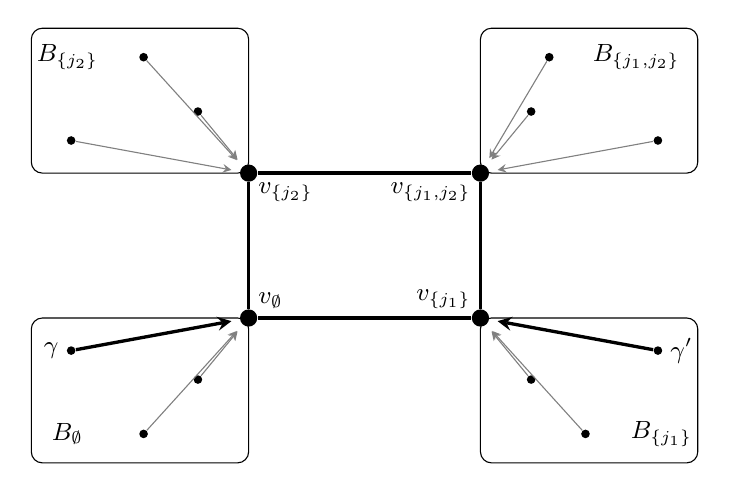
\begin{tikzpicture}[scale=0.92,
            st/.style={circle,fill=black,inner sep=1.1pt},
            vv/.style={circle,fill=black,inner sep=2.2pt},
            fun/.style={->,>=stealth,gray,shorten >=3pt},
            hl/.style={->,>=stealth,very thick,shorten >=3pt}]

            % the four blocks, meeting the central square at their inner corners
            \draw[rounded corners=4pt] (-4.6,-3.0) rectangle (-1.6,-1.0);
            \draw[rounded corners=4pt] ( 1.6,-3.0) rectangle ( 4.6,-1.0);
            \draw[rounded corners=4pt] (-4.6, 1.0) rectangle (-1.6, 3.0);
            \draw[rounded corners=4pt] ( 1.6, 1.0) rectangle ( 4.6, 3.0);
            \node at (-4.1,-2.60) {\small$B_\emptyset$};
            \node at ( 4.1,-2.60) {\small$B_{\{j_1\}}$};
            \node at (-4.1, 2.60) {\small$B_{\{j_2\}}$};
            \node at ( 3.75, 2.60) {\small$B_{\{j_1,j_2\}}$};

            % segment (ii): the hypercube, exactly the gap between the blocks
            \node[vv] (v00) at (-1.6,-1.0) {};
            \node[vv] (v10) at ( 1.6,-1.0) {};
            \node[vv] (v01) at (-1.6, 1.0) {};
            \node[vv] (v11) at ( 1.6, 1.0) {};
            \draw[very thick] (v00)--(v10) (v00)--(v01)
            (v10)--(v11) (v01)--(v11);
            \node[above right=0pt] at (v00) {\small$v_\emptyset$};
            \node[above left =0pt] at (v10) {\small$v_{\{j_1\}}$};
            \node[below right=0pt] at (v01) {\small$v_{\{j_2\}}$};
            \node[below left =0pt] at (v11) {\small$v_{\{j_1,j_2\}}$};

            % segments (i) and (iii): F_lambda funnels each block onto its v_J
            \node[st] (a1) at (-4.05,-1.45) {}; \node[left =1pt] at (a1) {\small$\gamma$};
            \node[st] (a2) at (-3.05,-2.60) {};
            \node[st] (a3) at (-2.30,-1.85) {};
            \node[st] (b1) at ( 4.05,-1.45) {}; \node[right=1pt] at (b1) {\small$\gamma'$};
            \node[st] (b2) at ( 3.05,-2.60) {};
            \node[st] (b3) at ( 2.30,-1.85) {};
            \node[st] (c1) at (-4.05, 1.45) {}; \node[st] (c2) at (-3.05, 2.60) {};
            \node[st] (c3) at (-2.30, 1.85) {};
            \node[st] (d1) at ( 4.05, 1.45) {}; \node[st] (d2) at ( 2.55, 2.60) {};
            \node[st] (d3) at ( 2.30, 1.85) {};

            \draw[fun] (a2)--(v00); \draw[fun] (a3)--(v00);
            \draw[fun] (b2)--(v10); \draw[fun] (b3)--(v10);
            \draw[fun] (c1)--(v01); \draw[fun] (c2)--(v01); \draw[fun] (c3)--(v01);
            \draw[fun] (d1)--(v11); \draw[fun] (d2)--(v11); \draw[fun] (d3)--(v11);
            \draw[hl]  (a1)--(v00); \draw[hl]  (b1)--(v10);
        \end{tikzpicture}
        \caption{\cref{def:flowens} at $k_\lambda=2$: arrows are steps of
            $F_\lambda$, funnelling each block $B_J$ onto $v_J$; the four $v_J$
            carry the hypercube $\{0,1\}^{k_\lambda}$ of segment~(ii).}
        \label{fig:flow}
    \end{figure}


    See \cref{fig:flow}. Segment~(ii) is legitimate: each $v_{J''}$ is a
    subset of $\gamma^{\ast}$, hence lies in $\mathscr{M}(s_0)$, and consecutive
    ones differ by one flip. The ensemble is \emph{not} memoryless, which is why
    the precedent machinery of \cref{sub:precG} applies to its first and
    third segments only.

    \begin{definition}[Hypercube congestion]
        \label{def:rholam}
        With $\bar\pi_\lambda$ as in~\eqref{eq:blocks}, put
        \begin{equation}
            \label{eq:rholam}
            \varrho_\lambda\ \coloneq\ \max_{J,\,j\in C_\lambda}\
            \frac{1}{\min\{\bar\pi_\lambda(J),\bar\pi_\lambda(J\triangle
            \{j\})\}}
            \sum_{(J_1,J_2)}\bar\pi_\lambda(J_1)\bar\pi_\lambda(J_2),
        \end{equation}
        the inner sum being over the ordered pairs whose increasing-order path
        in $\{0,1\}^{k_\lambda}$ traverses the directed edge
        $(J,J\triangle\{j\})$.
    \end{definition}

    The congestion of the two-level ensemble now splits in two. Its first
    and third segments are the rules \ref{H:null}--\ref{H:del} of
    $\mathcal{G}_\lambda$, which \cref{th:dropG} already controls; its
    middle segment lives inside a single hypercube, and everything it costs
    is $\varrho_\lambda$.

    \begin{theorem}[Gap without commitment]
        \label{th:gapflow}
        Let $\lambda\in[0,1]$, assume \cref{ass:null} with an exponent $\eta$
        satisfying $p^{1-\eta}\leq\tfrac12$, and work on the good event. Then
        \begin{equation}
            \label{eq:gapflow}
            \mathrm{Gap}(\mathbf{P}_\lambda)\ \geq\
            \frac{1}{40\,p\,s_0\,(2s^{\ast}+1)\,\max\{1,\varrho_\lambda\}} .
        \end{equation}
    \end{theorem}

    \begin{corollary}[A gap outside the windows]
        \label{cor:gapwindow}
        Under the hypotheses of \cref{th:gapflow}, if $k_\lambda=0$ then
        \begin{equation}
            \label{eq:gapwindow}
            \mathrm{Gap}(\mathbf{P}_\lambda)\ \geq\
            \frac{1}{40\,p\,s_0\,(2s^{\ast}+1)} .
        \end{equation}
    \end{corollary}

    Indeed $C_\lambda=\emptyset$, so the maximum in~\eqref{eq:rholam} is over
    the empty set and $\max\{1,\varrho_\lambda\}=1$; equivalently, there is a
    single block $B_\emptyset=\mathscr{M}(s_0)$ and
    $\widetilde{\mathcal{T}}_\lambda$ is the ensemble generated by
    $F_\lambda$. The bound is better than \cref{lemma:gap} by a factor of
    order $s_0/s^{\ast}$: $\mathcal{G}_\lambda$ clears the covariates outside
    $\gamma^{\ast}$ before it touches the others and so never needs the
    exchange move, which is where the second factor $s_0$ came from. It holds
    in particular at $\lambda=0$, where $c^{-}_0=c^{+}_0=\emptyset$ and
    $F_0$ is the plain descent $\gamma\mapsto\gamma\setminus\max(\gamma)$.

    \begin{remark}[How often is $k_\lambda>0$]
        \label{rem:kmeasure}
        A covariate $j\in\gamma^{\ast}$ belongs to $C_\lambda$ exactly when
        \begin{equation*}
            \frac{\kappa\log p-\log(2s^{\ast})}{\psi_j^{+}}
            \ <\ \lambda\ <\
            \frac{\kappa\log p+\log(2s^{\ast})}{\psi_j^{-}} ,
        \end{equation*}
        an interval of length at most
        $\kappa\log p\,(\psi_j^{+}-\psi_j^{-})/(\psi_j^{-}\psi_j^{+})
        +\log(2s^{\ast})\{1/\psi_j^{-}+1/\psi_j^{+}\}$. Summing over
        $j\in\gamma^{\ast}$, the set $\{\lambda\in[0,1]:k_\lambda\geq1\}$ has
        Lebesgue measure at most that sum, which is
        $\mathcal{O}\bigl(s^{\ast}\log s^{\ast}/\min_j\psi_j^{-}\bigr)$ when
        the spreads $\psi_j^{+}-\psi_j^{-}$ are small compared with the
        $\psi_j^{-}$. So \cref{cor:gapwindow} applies for all
        but a short list of temperature windows, whose endpoints are
        computable in advance; a
        tempering schedule can be chosen to step across them.
    \end{remark}


    \subsection{When the undecided covariates do not interact}

    It remains to bound $\varrho_\lambda$, and here the near-neutrality of
    $C_\lambda$ enters. Everything depends on how far $\bar\pi_\lambda$ is
    from a product measure on $\{0,1\}^{k_\lambda}$.

    \begin{lemma}[Product measures are free]
        \label{lemma:prodfree}
        If $\bar\pi_\lambda$ is a product measure on
        $2^{C_\lambda}$, then $\varrho_\lambda\leq1$.
    \end{lemma}


    \begin{lemma}[Comparison]
        \label{lemma:comparison}
        Suppose there is a product measure $\bar\mu$ on $2^{C_\lambda}$
        with $\abs{\log\{\bar\pi_\lambda(J)/\bar\mu(J)\}}\leq D$ for every
        $J\subseteq C_\lambda$. Then $\varrho_\lambda\leq e^{3D}$.
    \end{lemma}


    The deviation $D$ is controlled by the interaction \emph{among the
    undecided covariates alone}:
    \begin{equation}
        \label{eq:DeltaC}
        \Delta^{C}_\lambda\ \coloneq\ \max_{j\in C_\lambda}\
        \max\bigl\{\abs{\psi_j(c^{-}_\lambda\cup U)
            -\psi_j(c^{-}_\lambda\cup U')}:\
        U,U'\subseteq C_\lambda\setminus\{j\}\bigr\} .
    \end{equation}

    \begin{proposition}[Bound on $\varrho_\lambda$]
        \label{prop:rhobound}
        Under the hypotheses of \cref{th:gapflow},
        \begin{equation}
            \label{eq:rhobound}
            \varrho_\lambda\ \leq\ \bigl\{2(2s^{\ast}+1)\bigr\}^{6}
            \exp\bigl\{6k_\lambda\Delta^{C}_\lambda\bigr\} .
        \end{equation}
    \end{proposition}


    \begin{remark}[What the flow buys]
        \label{rem:flowbuys}
        Combining \cref{th:gapflow} and \cref{prop:rhobound},
        \begin{equation}
            \label{eq:gapflowfinal}
            \mathrm{Gap}(\mathbf{P}_\lambda)\ \gtrsim\
            \frac{\exp\{-6k_\lambda\Delta^{C}_\lambda\}}
            {p\,s_0\,(s^{\ast})^{7}} ,
        \end{equation}
        against the $(1+k_\lambda\Theta_\lambda)^{k_\lambda}$ that the
        memoryless ensemble of \cref{sec:flow} would have charged. The two
        differ in what the exponent contains. There it is
        $k_\lambda\log(k_\lambda\Theta_\lambda)$ with
        $\Theta_\lambda\geq(2s^{\ast})^{-1}$ always, so the penalty is paid
        whenever $k_\lambda>0$, however benign the undecided covariates.
        In~\eqref{eq:gapflowfinal} it is $6k_\lambda\Delta^{C}_\lambda$, which
        vanishes when the undecided covariates do not interact
        \emph{with each other}, and then the bound is polynomial with no
        reference to $k_\lambda$ at all.

        This is the case that matters in practice. Undecided covariates are
        those with $\lambda\psi_j\approx\kappa\log p$, that is with nearly
        equal $\psi_j$; by \cref{lemma:forward}\ref{it:fs_a} and the
        transfer between $\psi_j$ and the explained energy, nearly equal
        $\psi_j$ means nearly equal $\abs{\beta^{\ast}_j}$. So $C_\lambda$ is
        typically a group of covariates with tied coefficients, and
        $\Delta^{C}_\lambda$ measures only how much those particular columns
        interact --- a $k_\lambda\times k_\lambda$ question, not an $s^{\ast}$
        or $s_0$ one. For a design whose $\beta^{\ast}$ takes two magnitudes,
        with multiplicities four and six,
        $\Delta^{C}_\lambda$ is the interaction among four or six independent
        Gaussian columns, which is $\mathcal{O}(1)$: a memoryless ensemble
        would charge $(1+6\Theta_\lambda)^{6}$ there, and \cref{th:gapflow}
        charges a constant.
    \end{remark}

    \bibliographystyle{imsart-nameyear}
    \bibliography{bvs}
    \appendix
    \section{Deferred proofs}
\label{sec:app}

% \begin{proof}[Proof of Lemma~\ref{lemma:master}]
%     Dividing numerator and denominator of the last fraction
%     in~\eqref{eq:Lik} by $g^{n/2}$, and writing $C_n(Y)$ for the
%     $\gamma$-free prefactor,
%     \begin{equation}
%         \label{eq:logL}
%         \log\mathcal{L}_n(Y\mid\gamma)
%         =\log C_n(Y)-\frac n2\log g
%         -\frac{\abs \gamma}{2}\log(1+g)
%         -\frac n2\log\bigl\{g^{-1}+1-R^{2}_\gamma\bigr\}.
%     \end{equation}
%     The first two terms of the right-hand side of~\eqref{eq:logL} do not
%     depend on $\gamma$, hence cancel in a difference:
%     \begin{equation}
%         \label{eq:logLratio}
%         \log\frac{\mathcal{L}_n(Y\mid\gamma)}
%         {\mathcal{L}_n(Y\mid\gamma')}
%         =\frac{\abs{\gamma'}-\abs \gamma}{2}\log(1+g)
%         +\frac n2\log\frac{g^{-1}+1-R^{2}_{\gamma'}}
%         {g^{-1}+1-R^{2}_{\gamma}} .
%     \end{equation}
%     By~\eqref{eq:prior} and~\eqref{eq:pilambda}, the normalising constants
%     cancelling,
%     \begin{equation*}
%         \log\frac{\pi_n^{(\lambda)}(\gamma\mid Y)}
%         {\pi_n^{(\lambda)}(\gamma'\mid Y)}
%         =\log\frac{\pi(\gamma)}{\pi(\gamma')}
%         +\lambda\log\frac{\mathcal{L}_n(Y\mid\gamma)}
%         {\mathcal{L}_n(Y\mid\gamma')}
%         =\kappa\bigl(\abs{\gamma'}-\abs \gamma\bigr)\log p
%         +\lambda\log\frac{\mathcal{L}_n(Y\mid\gamma)}
%         {\mathcal{L}_n(Y\mid\gamma')} .
%     \end{equation*}
%     Substituting~\eqref{eq:logLratio} and collecting the two terms
%     carrying the factor $\abs{\gamma'}-\abs \gamma$
%     gives~\eqref{eq:master}.
% \end{proof}

Every proof of the paper is collected here, together with the notation and
the deterministic bounds they rest on. Only the proof of \cref{th:drop}
involves the temperature, and it involves it only through the factor
$\lambda$ multiplying the fit term of~\eqref{eq:master}.

\subsection{Notation}
\label{sec:prelim}

We use throughout the effective noise of YWJ,
\begin{equation}
    \label{eq:wtilde}
    \widetilde w\ \coloneq\ X_{S^{c}}\beta^\ast_{S^{c}}+w,
    \qquad\text{so that}\qquad
    Y=\signal+\widetilde w ,
\end{equation}
the elementary inequalities
\begin{gather}
    \label{eq:elementary}
    \log(1+x)\leq x\ \ (x>-1),
    \qquad
    \norm{a+b}_2^{2}\leq2\norm a_2^{2}+2\norm b_2^{2},\\
    \nonumber
    \frac{a}{a+b}\geq\min\Bigl\{\frac12,\frac{a}{2b}\Bigr\}
    \ \ (a,b>0),
\end{gather}
and, for an underfitted $\gamma\in\mathscr{M}(s_0)$, the quantity
\begin{equation}
    \label{eq:Adef}
    A^{2}\ \coloneq\ \nu\,
    \frac{\norm{(I-\Phi_\gamma)\signal}_2^{2}}
    {\abs{\gamma^{\ast}\setminus\gamma}}\ >\ 0 ,
\end{equation}
the dependence on $\gamma$ being suppressed, as YWJ suppress it, since
$\gamma$ is fixed wherever $A$ occurs.


\subsection{Deterministic bounds}
\label{sub:appdet}

\begin{lemma}[Uniform residual lower bound]
    \label{lemma:residual}
    On the good event, and under~\eqref{eq:Dassumption}, every
    $\bar\gamma\in\mathscr{M}(s_0)$ satisfies
    \begin{equation}
        \label{eq:residual}
        \norm Y_2^{2}\bigl(g^{-1}+1-R^{2}_{\bar\gamma}\bigr)
        \ \geq\ \norm{(I-\Phi_{\bar\gamma})Y}_2^{2}
        \ \geq\ \frac{n\sigma_0^{2}}{8} .
    \end{equation}
\end{lemma}

\begin{proof}
    Since $\norm Y_2^{2}(g^{-1}+1-R^{2}_{\bar\gamma})
    =g^{-1}\norm Y_2^{2}+\norm{(I-\Phi_{\bar\gamma})Y}_2^{2}$, the first
    inequality amounts to discarding $g^{-1}\norm Y_2^{2}\geq0$. For the
    second, fix $\bar\gamma\in\mathscr{M}(s_0)$ and set
    $\bar\gamma^{+}\coloneq\bar\gamma\cup\gamma^{\ast}$, so that
    $\abs{\bar\gamma^{+}}\leq\abs{\bar\gamma}+s^{\ast}\leq s$ and
    $\bar\gamma^{+}\in\mathscr{M}(s)$. Since
    $\bar\gamma\subseteq\bar\gamma^{+}$, the range of $\Phi_{\bar\gamma}$
    is contained in that of $\Phi_{\bar\gamma^{+}}$, so
    $I-\Phi_{\bar\gamma}\succcurlyeq I-\Phi_{\bar\gamma^{+}}$ and
    \begin{equation}
        \label{eq:res1}
        \norm{(I-\Phi_{\bar\gamma})Y}_2^{2}
        \ \geq\ \norm{(I-\Phi_{\bar\gamma^{+}})Y}_2^{2}.
    \end{equation}
    Because $\gamma^{\ast}\subseteq\bar\gamma^{+}$, the vector $\signal$
    lies in the range of $\Phi_{\bar\gamma^{+}}$, so
    $(I-\Phi_{\bar\gamma^{+}})\signal=0$ and
    \begin{equation*}
    (I-\Phi_{\bar\gamma^{+}})
        Y
        =(I-\Phi_{\bar\gamma^{+}})w
        +(I-\Phi_{\bar\gamma^{+}})X_{S^{c}}\beta^\ast_{S^{c}} .
    \end{equation*}
    Apply $\norm{a+b}_2^{2}\geq\tfrac12\norm a_2^{2}-\norm b_2^{2}$, which
    is the rearrangement of $\tfrac12(\norm a_2-2\norm b_2)^{2}\geq0$,
    with $a=(I-\Phi_{\bar\gamma^{+}})w$ and
    $b=(I-\Phi_{\bar\gamma^{+}})X_{S^{c}}\beta^\ast_{S^{c}}$. Since
    projections are non-expansive, $\norm b_2^{2}\leq
    \norm{X_{S^{c}}\beta^\ast_{S^{c}}}_2^{2}\leq\Ltil\sigma_0^{2}\log p$
    by \cref{ass:A}, and $\norm a_2^{2}=\norm w_2^{2}
    -w^{\top}\Phi_{\bar\gamma^{+}}w$ because $I-\Phi_{\bar\gamma^+}$ is a
    projection. Hence
    \begin{equation*}
        \norm{(I-\Phi_{\bar\gamma^{+}})Y}_2^{2}
        \ \geq\ \tfrac12\bigl(\norm w_2^{2}
        -w^{\top}\Phi_{\bar\gamma^{+}}w\bigr)
        -\Ltil\sigma_0^{2}\log p .
    \end{equation*}
    On $\mathcal{C}_n$ we have $\norm w_2^{2}\geq n\sigma_0^{2}/2$, and on
    $\mathcal{B}_n$, applied to $\bar\gamma^{+}\in\mathscr{M}(s)$, we have
    $w^{\top}\Phi_{\bar\gamma^{+}}w\leq 8s\,\sigma_0^{2}\log p$.
    Therefore
    \begin{equation*}
        \norm{(I-\Phi_{\bar\gamma^{+}})Y}_2^{2}
        \ \geq\ \frac{n\sigma_0^{2}}{4}
        -\bigl\{4s+\Ltil\bigr\}\sigma_0^{2}\log p
        \ \geq\ \frac{n\sigma_0^{2}}{4}
        -\bigl\{8s+\Ltil\bigr\}\sigma_0^{2}\log p ,
    \end{equation*}
    and by~\eqref{eq:Dassumption} the subtracted term is at most
    $n\sigma_0^{2}/32$, so the right-hand side is at least
    $7n\sigma_0^{2}/32\geq n\sigma_0^{2}/8$. Combining
    with~\eqref{eq:res1} finishes the proof.
\end{proof}

\begin{lemma}[Effective noise]
    \label{lemma:noise}
    On the good event, and under~\eqref{eq:Dassumption}:
    \begin{equivcond}
        \item\label{it:noise_i}
        $\norm{\widetilde w}_2^{2}\leq2\Ltil\sigma_0^{2}\log p
        +3n\sigma_0^{2}$;
        \item\label{it:noise_ii} for every pair
        $\gamma_2\subset\gamma_1$ of $\mathscr{M}(s)$ with
        $\abs{\gamma_1}-\abs{\gamma_2}=1$,
        \begin{equation*}
            \norm{(\Phi_{\gamma_1}-\Phi_{\gamma_2})\widetilde w}_2^{2}
            \ \leq\ 2(L+\Ltil)\,\sigma_0^{2}\log p
            \ \leq\ \frac{n\nu^{2}C_\beta^{2}}{64} .
        \end{equation*}
    \end{equivcond}
\end{lemma}

\begin{proof}
    \ref{it:noise_i} By~\eqref{eq:elementary} and \cref{ass:A},
    $\norm{\widetilde w}_2^{2}\leq2\norm{X_{S^{c}}
        \beta^\ast_{S^{c}}}_2^{2}+2\norm w_2^{2}
    \leq2\Ltil\sigma_0^{2}\log p+2\norm w_2^{2}$, and on $\mathcal{C}_n$
    we have $\norm w_2^{2}\leq\tfrac32n\sigma_0^{2}$.

    \ref{it:noise_ii} Write $\Pi=\Phi_{\gamma_1}-\Phi_{\gamma_2}$, an
    orthogonal projection, so that $\norm{\Pi v}_2\leq\norm v_2$ for every
    $v$ and $\norm{\Pi w}_2^{2}=w^{\top}\Pi w$. Hence,
    by~\eqref{eq:elementary},
    \begin{align*}
        \norm{\Pi\widetilde w}_2^{2}
        &\leq2\norm{\Pi X_{S^{c}}\beta^\ast_{S^{c}}}_2^{2}
        +2\norm{\Pi w}_2^{2}
        \leq2\norm{X_{S^{c}}\beta^\ast_{S^{c}}}_2^{2}
        +2\,w^{\top}\bigl(\Phi_{\gamma_1}-\Phi_{\gamma_2}\bigr)w\\
        &\leq2\Ltil\sigma_0^{2}\log p+2L\sigma_0^{2}\log p,
    \end{align*}
    using \cref{ass:A} for the first term and the event $\mathcal{A}_n$,
    applied to the nested pair $\gamma_2\subset\gamma_1$ of
    $\mathscr{M}(s)$ with $\abs{\gamma_1}-\abs{\gamma_2}=1$, for the
    second. The final inequality is \cref{ass:betamin} rearranged.
\end{proof}

\begin{lemma}[Upper bound on the regularised residual]
    \label{lemma:Dupper}
    On the good event, and under~\eqref{eq:Dassumption} and $n\geq3$, every
    $\gamma\in\mathscr{M}(s_0)$ satisfies
    \begin{equation}
        \label{eq:Dupper}
        \norm Y_2^{2}\bigl(g^{-1}+1-R^{2}_{\gamma}\bigr)
        \ \leq\ 2\norm{(I-\Phi_\gamma)\signal}_2^{2}
        +8\,n\sigma_0^{2} .
    \end{equation}
\end{lemma}

\begin{proof}
    By~\eqref{eq:wtilde} and~\eqref{eq:elementary},
    \begin{equation*}
        \norm{(I-\Phi_\gamma)Y}_2^{2}
        \leq2\norm{(I-\Phi_\gamma)\signal}_2^{2}
        +2\norm{(I-\Phi_\gamma)\widetilde w}_2^{2}
        \leq2\norm{(I-\Phi_\gamma)\signal}_2^{2}
        +2\norm{\widetilde w}_2^{2},
    \end{equation*}
    the last step because $I-\Phi_\gamma$ is a projection. By
    \cref{lemma:noise}\ref{it:noise_i}, $2\norm{\widetilde w}_2^{2}\leq
    4\Ltil\sigma_0^{2}\log p+6n\sigma_0^{2}$, and on $\mathcal{D}_n$ we
    have $g^{-1}\norm Y_2^{2}\leq(2\log p+3)\sigma_0^{2}$. Adding the two,
    the additive term is at most
    \begin{equation*}
        \bigl\{4\Ltil\log p+6n+2\log p+3\bigr\}\sigma_0^{2}
        \ \leq\ \Bigl\{\frac n8+6n+\frac{n}{128}+n\Bigr\}\sigma_0^{2}
        \ \leq\ 8n\sigma_0^{2},
    \end{equation*}
    where we used, in order: $\Ltil\log p\leq n/32$
    from~\eqref{eq:Dassumption}, whence $4\Ltil\log p\leq n/8$; the same display
    with $\Ltil$ replaced by $8s\geq8$, whence $\log p\leq n/256$ and
    $2\log p\leq n/128$; and $3\leq n$.
\end{proof}

\begin{lemma}[Greedy selection; YWJ, Lemma~8]
    \label{lemma:forward}
    Let $\gamma\in\mathscr{M}(s_0)$ be underfitted and let $j_\gamma$ be
    as in~\eqref{eq:jdef}. Under \cref{ass:B,ass:D,ass:betamin}:
    \begin{equivcond}
        \item\label{it:fs_a}
        $\norm{(\Phi_{\gamma\cup\{j_\gamma\}}-\Phi_\gamma)
            \signal}_2^{2}\geq A^{2}$, and moreover
        \begin{equation}
            \label{eq:Alower}
            A^{2}\ \geq\ n\,\nu^{2}\min_{j\in\gamma^{\ast}}
            \abs{\beta^\ast_j}^{2}
            \ \geq\ n\,\nu^{2}C_\beta^{2} ;
        \end{equation}
        \item\label{it:fs_b} if in addition $\gamma$ is saturated and
        $k_\gamma$ is as in~\eqref{eq:kdef}, then, with
        $\widetilde\gamma=\gamma\cup\{j_\gamma\}$ and
        $\gamma'=\widetilde\gamma\setminus\{k_\gamma\}$,
        \begin{equation*}
            \norm{(\Phi_{\widetilde\gamma}-\Phi_{\gamma'})
                \signal}_2^{2}
            \ \leq\ n\,\omega(X)\,
            \frac{\norm{\beta^\ast_{\gamma^{\ast}\setminus\gamma}}_2^{2}}
            {s_0-s^{\ast}}
            \ \leq\ \frac{A^{2}}{4} .
        \end{equation*}
    \end{equivcond}
\end{lemma}

\begin{proof}
    We use two facts from YWJ. The first is their Lemma~7, the rank-one
    update formula: for $\bar\gamma\in\mathscr{M}(s)$ and
    $k\notin\bar\gamma$ with $\abs{\bar\gamma}<s$,
    \begin{equation}
        \label{eq:rankone}
        \Phi_{\bar\gamma\cup\{k\}}-\Phi_{\bar\gamma}
        =\frac{(I-\Phi_{\bar\gamma})X_kX_k^{\top}
            (I-\Phi_{\bar\gamma})}
        {X_k^{\top}(I-\Phi_{\bar\gamma})X_k},
    \end{equation}
    which follows from the block inversion formula applied to
    $X_{\bar\gamma\cup\{k\}}^{\top}X_{\bar\gamma\cup\{k\}}$. The second
    is their Lemma~6: under \cref{ass:B}, for every nested pair
    $\gamma_2\subset\gamma_1$ of $\mathscr{M}(s)$,
    \begin{equation}
        \label{eq:underfit}
        \lambda_{\min}\Bigl(\frac1n
        X_{\gamma_1\setminus\gamma_2}^{\top}
        (I-\Phi_{\gamma_2})X_{\gamma_1\setminus\gamma_2}\Bigr)
        \ \geq\ \nu ,
    \end{equation}
    because the matrix inside is $n$ times the Schur complement of the
    block $X_{\gamma_2}^{\top}X_{\gamma_2}$ in
    $X_{\gamma_1}^{\top}X_{\gamma_1}$, hence its inverse is the
    corresponding diagonal block of
    $(n^{-1}X_{\gamma_1}^{\top}X_{\gamma_1})^{-1}$, whose largest
    eigenvalue is at most
    $\lambda_{\min}(n^{-1}X_{\gamma_1}^{\top}X_{\gamma_1})^{-1}
    \leq\nu^{-1}$.

    \emph{Proof of~\ref{it:fs_a}.} Put $u\coloneq(I-\Phi_\gamma)\signal$.
    For $\ell\in\gamma^{\ast}\setminus\gamma$, idempotence of projections
    and~\eqref{eq:rankone} give
    \begin{align}
        \notag
        \norm{\Phi_{\gamma\cup\{\ell\}}\signal}_2^{2}
        -\norm{\Phi_{\gamma}\signal}_2^{2}
        &=(\beta^\ast_{\gamma^{\ast}})^{\top}
        X_{\gamma^{\ast}}^{\top}
        \bigl(\Phi_{\gamma\cup\{\ell\}}-\Phi_\gamma\bigr)\signal\\
        \label{eq:onegain}
        &=\frac{\langle X_\ell,u\rangle^{2}}
        {X_\ell^{\top}(I-\Phi_\gamma)X_\ell}
        \ \geq\ \frac{\langle X_\ell,u\rangle^{2}}{n},
    \end{align}
    where the last step uses
    $X_\ell^{\top}(I-\Phi_\gamma)X_\ell\leq\norm{X_\ell}_2^{2}=n$ and,
    for the middle equality, that
    $X_\ell^{\top}(I-\Phi_\gamma)\signal=\langle X_\ell,u\rangle$.
    Summing~\eqref{eq:onegain} over $\ell\in\gamma^{\ast}\setminus\gamma$,
    \begin{equation}
        \label{eq:sumgain}
        \sum_{\ell\in\gamma^{\ast}\setminus\gamma}
        \Bigl\{\norm{\Phi_{\gamma\cup\{\ell\}}\signal}_2^{2}
        -\norm{\Phi_{\gamma}\signal}_2^{2}\Bigr\}
        \ \geq\ \frac1n
        \norm{X_{\gamma^{\ast}\setminus\gamma}^{\top}u}_2^{2}
        \ =\ \frac1n\norm{X_{\gamma^{\ast}\cup\gamma}^{\top}u}_2^{2},
    \end{equation}
    the last equality because $X_j^{\top}u=0$ for $j\in\gamma$: indeed
    $X_j$ lies in the range of $\Phi_\gamma$, to which $u$ is orthogonal
    by construction. Now $u$ lies in the range of
    $X_{\gamma^{\ast}\cup\gamma}$, so $u=X_{\gamma^{\ast}\cup\gamma}v$ for
    some $v$; writing
    $M\coloneq X_{\gamma^{\ast}\cup\gamma}^{\top}
    X_{\gamma^{\ast}\cup\gamma}$, we have
    $\abs{\gamma^{\ast}\cup\gamma}\leq s$, hence $M\succcurlyeq n\nu I$ by
    \cref{ass:B}, and therefore
    \begin{equation*}
        \frac1n\norm{X_{\gamma^{\ast}\cup\gamma}^{\top}u}_2^{2}
        =\frac1nv^{\top}M^{2}v
        \ \geq\ \nu\,v^{\top}Mv
        =\nu\norm u_2^{2},
    \end{equation*}
    the inequality because $M^{2}-n\nu M=M^{1/2}(M-n\nu I)M^{1/2}
    \succcurlyeq0$. Combining with~\eqref{eq:sumgain} and dividing by
    $\abs{\gamma^{\ast}\setminus\gamma}$, the maximum over $\ell$ of the
    left-hand side of~\eqref{eq:onegain} is at least
    $\nu\norm u_2^{2}/\abs{\gamma^{\ast}\setminus\gamma}=A^{2}$. Since
    $j_\gamma$ attains that maximum by~\eqref{eq:jdef}, and since the
    left-hand side of~\eqref{eq:onegain} equals
    $\norm{(\Phi_{\gamma\cup\{\ell\}}-\Phi_\gamma)\signal}_2^{2}$ by
    idempotence, the first claim follows.

    For~\eqref{eq:Alower}, note that
    $(I-\Phi_\gamma)\signal=(I-\Phi_\gamma)
    X_{\gamma^{\ast}\setminus\gamma}
    \beta^\ast_{\gamma^{\ast}\setminus\gamma}$, because the columns $X_j$
    with $j\in\gamma^{\ast}\cap\gamma$ lie in the range of $\Phi_\gamma$;
    hence by~\eqref{eq:underfit} applied to
    $\gamma\subset\gamma^{\ast}\cup\gamma$,
    \begin{equation}
        \label{eq:usquare}
        \norm u_2^{2}
        =(\beta^\ast_{\gamma^{\ast}\setminus\gamma})^{\top}
        X_{\gamma^{\ast}\setminus\gamma}^{\top}(I-\Phi_\gamma)
        X_{\gamma^{\ast}\setminus\gamma}
        \beta^\ast_{\gamma^{\ast}\setminus\gamma}
        \ \geq\ n\,\nu
        \norm{\beta^\ast_{\gamma^{\ast}\setminus\gamma}}_2^{2},
    \end{equation}
    so that, using
    $\norm{\beta^\ast_{\gamma^{\ast}\setminus\gamma}}_2^{2}
    \geq\abs{\gamma^{\ast}\setminus\gamma}
    \min_{j\in\gamma^{\ast}}\abs{\beta^\ast_j}^{2}$ and~\eqref{eq:S},
    \begin{equation}
        \label{eq:Achain}
        A^{2}=\frac{\nu\norm u_2^{2}}
        {\abs{\gamma^{\ast}\setminus\gamma}}
        \ \geq\ \frac{n\nu^{2}
            \norm{\beta^\ast_{\gamma^{\ast}\setminus\gamma}}_2^{2}}
        {\abs{\gamma^{\ast}\setminus\gamma}}
        \ \geq\ n\nu^{2}\min_{j\in\gamma^{\ast}}
        \abs{\beta^\ast_j}^{2}
        \ \geq\ n\nu^{2}C_\beta^{2} .
    \end{equation}

    \emph{Proof of~\ref{it:fs_b}.} Write
    $\widetilde\gamma=\gamma\cup\{j_\gamma\}$. For
    $\bar\gamma\in\mathscr{M}(s)$ let $\widehat\beta(\bar\gamma)$ solve
    \begin{equation}
        \label{eq:modLS}
        \min\bigl\{\norm{X\beta
        -X_{\gamma^{\ast}\setminus\widetilde\gamma}
            \beta^\ast_{\gamma^{\ast}\setminus\widetilde\gamma}}_2^{2}:\
        \beta\in\bbR^{p},\ \beta_j=0\ \text{for }j\notin\bar\gamma\bigr\},
    \end{equation}
    so that
    \begin{equation}
        \label{eq:LSid}
        \norm{X\widehat\beta(\bar\gamma)
        -X_{\gamma^{\ast}\setminus\widetilde\gamma}
            \beta^\ast_{\gamma^{\ast}\setminus\widetilde\gamma}}_2^{2}
        =\norm{(I-\Phi_{\bar\gamma})
            X_{\gamma^{\ast}\setminus\widetilde\gamma}
            \beta^\ast_{\gamma^{\ast}\setminus\widetilde\gamma}}_2^{2},
        \qquad
        \widehat\beta(\bar\gamma)_{\bar\gamma}
        =(X_{\bar\gamma}^{\top}X_{\bar\gamma})^{-1}X_{\bar\gamma}^{\top}
        X_{\gamma^{\ast}\setminus\widetilde\gamma}
        \beta^\ast_{\gamma^{\ast}\setminus\widetilde\gamma} .
    \end{equation}
    Since
    $k_\gamma\notin\gamma^\ast$ we have
    $\Phi_{\widetilde\gamma}X_{\gamma^{\ast}\cap\widetilde\gamma}
    =\Phi_{\widetilde\gamma\setminus\{k\}}
    X_{\gamma^{\ast}\cap\widetilde\gamma}$ for every
    $k\in\widetilde\gamma\setminus\gamma^{\ast}$, so with
    $\gamma'=\widetilde\gamma\setminus\{k_\gamma\}$
    \begin{align}
        \notag
        \norm{(\Phi_{\widetilde\gamma}-\Phi_{\gamma'})
            \signal}_2^{2}
        &=\norm{(\Phi_{\widetilde\gamma}-\Phi_{\gamma'})
            X_{\gamma^{\ast}\setminus\widetilde\gamma}
            \beta^\ast_{\gamma^{\ast}\setminus\widetilde\gamma}}_2^{2}\\
        \notag
        &=\norm{(I-\Phi_{\gamma'})
            X_{\gamma^{\ast}\setminus\widetilde\gamma}
            \beta^\ast_{\gamma^{\ast}\setminus\widetilde\gamma}}_2^{2}
        -\norm{(I-\Phi_{\widetilde\gamma})
            X_{\gamma^{\ast}\setminus\widetilde\gamma}
            \beta^\ast_{\gamma^{\ast}\setminus\widetilde\gamma}}_2^{2}\\
        \label{eq:LSdiff}
        &=\norm{X\widehat\beta(\gamma')
        -X_{\gamma^{\ast}\setminus\widetilde\gamma}
            \beta^\ast_{\gamma^{\ast}\setminus\widetilde\gamma}}_2^{2}
        -\norm{X\widehat\beta(\widetilde\gamma)
        -X_{\gamma^{\ast}\setminus\widetilde\gamma}
            \beta^\ast_{\gamma^{\ast}\setminus\widetilde\gamma}}_2^{2},
    \end{align}
    using in the second line that
    $\Phi_{\widetilde\gamma}-\Phi_{\gamma'}$ is a projection and
    $\gamma'\subset\widetilde\gamma$. By optimality of
    $\widehat\beta(\widetilde\gamma)$ in~\eqref{eq:modLS}, the residual
    $X\widehat\beta(\widetilde\gamma)
    -X_{\gamma^{\ast}\setminus\widetilde\gamma}
    \beta^\ast_{\gamma^{\ast}\setminus\widetilde\gamma}$ is orthogonal to
    $X_k$ for every $k\in\widetilde\gamma$, so for such $k$
    \begin{align*}
        \norm{X\widehat\beta(\widetilde\gamma\setminus\{k\})
        -X_{\gamma^{\ast}\setminus\widetilde\gamma}
            \beta^\ast_{\gamma^{\ast}\setminus\widetilde\gamma}}_2^{2}
        &\ \leq\ \norm{X\widehat\beta(\widetilde\gamma)
        -X_{\gamma^{\ast}\setminus\widetilde\gamma}
            \beta^\ast_{\gamma^{\ast}\setminus\widetilde\gamma}
            -X_k\widehat\beta_k(\widetilde\gamma)}_2^{2}\\
        &\ =\ \norm{X\widehat\beta(\widetilde\gamma)
        -X_{\gamma^{\ast}\setminus\widetilde\gamma}
            \beta^\ast_{\gamma^{\ast}\setminus\widetilde\gamma}}_2^{2}
        +\norm{X_k}_2^{2}\,
        \abs{\widehat\beta_k(\widetilde\gamma)}^{2},
    \end{align*}
    the first line because the vector $\widehat\beta(\widetilde\gamma)$
    with its $k$th coordinate zeroed is feasible for the problem defining
    $\widehat\beta(\widetilde\gamma\setminus\{k\})$, and the second by
    orthogonality. Since $\norm{X_k}_2^{2}=n$ and $k_\gamma$ minimises the
    left-hand side over $k\in\gamma\setminus\gamma^\ast
    =\widetilde\gamma\setminus(\gamma^{\ast}\cup\{j_\gamma\})$, whose
    cardinality is $s_0-\abs{\gamma\cap\gamma^{\ast}}\geq s_0-s^{\ast}$,
    \begin{equation*}
        \norm{X\widehat\beta(\gamma')
        -X_{\gamma^{\ast}\setminus\widetilde\gamma}
            \beta^\ast_{\gamma^{\ast}\setminus\widetilde\gamma}}_2^{2}
        -\norm{X\widehat\beta(\widetilde\gamma)
        -X_{\gamma^{\ast}\setminus\widetilde\gamma}
            \beta^\ast_{\gamma^{\ast}\setminus\widetilde\gamma}}_2^{2}
        \ \leq\ n\min_{k\in\gamma\setminus\gamma^\ast}
        \abs{\widehat\beta_k(\widetilde\gamma)}^{2}
        \ \leq\ \frac{n\norm{\widehat\beta(\widetilde\gamma)}_2^{2}}
        {s_0-s^{\ast}},
    \end{equation*}
    a minimum being at most the average. Finally
    \begin{equation*}
        \norm{\widehat\beta(\widetilde\gamma)}_2^{2}
        =\norm{(X_{\widetilde\gamma}^{\top}X_{\widetilde\gamma})^{-1}
            X_{\widetilde\gamma}^{\top}
            X_{\gamma^{\ast}\setminus\widetilde\gamma}
            \beta^\ast_{\gamma^{\ast}\setminus\widetilde\gamma}}_2^{2}
        \ \leq\ \omega(X)\,
        \norm{\beta^\ast_{\gamma^{\ast}
        \setminus\widetilde\gamma}}_2^{2}
        \ \leq\ \omega(X)\,
        \norm{\beta^\ast_{\gamma^{\ast}\setminus\gamma}}_2^{2},
    \end{equation*}
    by the definition of $\omega(X)$ in \cref{ass:D} and
    $\gamma^{\ast}\setminus\widetilde\gamma\subseteq
    \gamma^{\ast}\setminus\gamma$. Together with~\eqref{eq:LSdiff} this
    gives the first inequality of~\ref{it:fs_b}.

    For the second, combine
    $A^{2}\geq n\nu^{2}
    \norm{\beta^\ast_{\gamma^{\ast}\setminus\gamma}}_2^{2}/
    \abs{\gamma^{\ast}\setminus\gamma}\geq
    n\nu^{2}\norm{\beta^\ast_{\gamma^{\ast}\setminus\gamma}}_2^{2}/
    s^{\ast}$, which is~\eqref{eq:Achain}, with the first inequality of
    \cref{ass:D}: $s_0\geq(4\nu^{-2}\omega(X)+1)s^{\ast}$ is equivalent to
    $4\omega(X)s^{\ast}\leq\nu^{2}(s_0-s^{\ast})$, that is to
    \begin{equation*}
        \frac{n\,\omega(X)
        \norm{\beta^\ast_{\gamma^{\ast}\setminus\gamma}}_2^{2}}
        {s_0-s^{\ast}}
        \ \leq\ \frac14\cdot
        \frac{n\,\nu^{2}
            \norm{\beta^\ast_{\gamma^{\ast}\setminus\gamma}}_2^{2}}
        {s^{\ast}}
        \ \leq\ \frac{A^{2}}{4} . \qedhere
    \end{equation*}
\end{proof}


\begin{remark}
    \label{rem:ywj_constant}
    With their constant $2$ in place of our $4$ in~\eqref{eq:Dassumption},
    YWJ obtain $\norm{v_2}_2\leq A/\sqrt2$ rather than
    $\norm{v_2}_2\leq A/2$, and combine it with a noise bound $A/4$. The
    resulting numbers do not close: on their page~2527 the displayed lower
    bound $A(A-A/4)-(A/\sqrt2)(A/\sqrt2+A/4)-A^{2}/16$ equals
    $0.0107\,A^{2}$, not the $A^{2}/8$ claimed, and it is negative if one
    keeps the factor $2$ that their own preceding display carries on the
    cross terms. Strengthening \cref{ass:D} to
    $s_0\geq(4\nu^{-2}\omega(X)+1)s^{\ast}$, and \cref{ass:betamin} so
    that the noise budget is $A/8$ rather than $A/4$, repairs this with
    room to spare; see~\eqref{eq:satdrop} below. Nothing else in their
    argument, or in ours, is affected.
\end{remark}

\begin{lemma}[Proxy bound]
    \label{lemma:proxy}
    For every $\gamma\in\mathscr{M}(s)$ and every
    $j\in\gamma\setminus\gamma^{\ast}$,
    \begin{equation}
        \label{eq:proxy}
        \bigl\|(\Phi_{\gamma}-\Phi_{\gamma\setminus\{j\}})
        \signal\bigr\|_2^{2}
        \ \leq\ n\,\omega(X)\,
        \bigl\|\beta^{\ast}_{\gamma^{\ast}\setminus\gamma}\bigr\|_2^{2} .
    \end{equation}
\end{lemma}

\begin{proof}
    This is the chain of displays in the proof of
    \cref{lemma:forward}\ref{it:fs_b}, run with $\widetilde\gamma$
    replaced by $\gamma$ and $k_\gamma$ by $j$. Every step used only
    $j\notin\gamma^{\ast}$ and $\gamma\in\mathscr{M}(s)$: first
    $\Phi_{\gamma}X_{\gamma^{\ast}\cap\gamma}
    =\Phi_{\gamma\setminus\{j\}}X_{\gamma^{\ast}\cap\gamma}$, so the left
    side equals $\|(\Phi_\gamma-\Phi_{\gamma\setminus\{j\}})
    X_{\gamma^{\ast}\setminus\gamma}
    \beta^{\ast}_{\gamma^{\ast}\setminus\gamma}\|_2^{2}$; then the
    identification with a difference of least-squares residuals; then
    feasibility of zeroing the $j$th coordinate, which gives the bound
    $n\abs{\widehat\beta_j(\gamma)}^{2}$; then
    $\|\widehat\beta(\gamma)\|_2^{2}\leq\omega(X)
    \|\beta^{\ast}_{\gamma^{\ast}\setminus\gamma}\|_2^{2}$. Taking
    $\gamma\supseteq\gamma^{\ast}$ makes the right side vanish and
    recovers the identity used in \cref{sub:over}.
\end{proof}

\subsection{Counting and paths}
\label{sub:appcount}

\begin{lemma}[Counting precedents]
    \label{lemma:count}
    Let $\bar\eta\in\mathscr{M}(s_0)$.
    \begin{equivcond}
        \item\label{it:cnt_i} $\mathcal{G}$ maps overfitted states to
        states containing $\gamma^{\ast}$. Consequently, if $\gamma$ is
        underfitted then every $\bar\gamma\in\Lambda(\gamma)$ is
        underfitted.
        \item\label{it:cnt_ii} $\bar\eta$ has at most $(s^{\ast}+1)p$
        immediate precedents that are underfitted --- that is, states
        $\bar\gamma\neq\bar\eta$ with
        $\mathcal{G}(\bar\gamma)=\bar\eta$ and $\bar\gamma$ underfitted
        --- and at most $p$ that are overfitted.
        \item\label{it:cnt_iii} Hence, for every $k\geq0$, the number of
        $\bar\gamma$ with $\mathcal{G}^{k}(\bar\gamma)=\bar\eta$ and
        $\bar\gamma,\mathcal{G}(\bar\gamma),\dots,
        \mathcal{G}^{k-1}(\bar\gamma)$ all underfitted is at most
        $\{(s^{\ast}+1)p\}^{k}$; and if
        $\bar\eta\supseteq\gamma^{\ast}$, the number of overfitted
        $\bar\gamma\in\Lambda_k(\bar\eta)$ is at most $p^{k}$.
    \end{equivcond}
\end{lemma}

\begin{proof}
    \ref{it:cnt_i} An overfitted $\bar\gamma$ is treated by
    rule~\ref{G:del}, which deletes
    $\ell_{\bar\gamma}\in\bar\gamma\setminus\gamma^{\ast}$ and therefore
    leaves $\gamma^{\ast}\subseteq\mathcal{G}(\bar\gamma)$; and
    $\gamma^{\ast}$ is a fixed point. So
    $\mathcal{G}^{k}(\bar\gamma)\supseteq\gamma^{\ast}$ for every
    $k\geq0$, and no such state is underfitted.

    \ref{it:cnt_ii} Let $\bar\gamma\neq\bar\eta$ be underfitted with
    $\mathcal{G}(\bar\gamma)=\bar\eta$. If rule~\ref{G:add} applies then
    $\bar\eta=\bar\gamma\cup\{j_{\bar\gamma}\}$ with
    $j_{\bar\gamma}\in\gamma^{\ast}$, so
    $\bar\gamma=\bar\eta\setminus\{j\}$ for some
    $j\in\gamma^{\ast}\cap\bar\eta$: at most $s^{\ast}$ states. If
    rule~\ref{G:exch} applies then
    $\bar\eta=\bar\gamma\cup\{j_{\bar\gamma}\}
    \setminus\{k_{\bar\gamma}\}$ with $j_{\bar\gamma}\in\gamma^{\ast}$
    and $k_{\bar\gamma}\in S^{c}$, so
    $\bar\gamma=\bar\eta\cup\{k\}\setminus\{j\}$ with
    $j\in\gamma^{\ast}\cap\bar\eta$ and $k\in S^{c}$: at most
    $s^{\ast}(p-s^{\ast})$ states. The total is at most
    $s^{\ast}(1+p-s^{\ast})\leq s^{\ast}(1+p)\leq(s^{\ast}+1)p$, the last
    step because $s^{\ast}\leq p$. If instead $\bar\gamma$ is overfitted
    then rule~\ref{G:del} applies and $\bar\gamma=\bar\eta\cup\{\ell\}$
    with $\ell\in S^{c}$: at most $p$ states.

    \ref{it:cnt_iii} Iterate~\ref{it:cnt_ii}: a state counted at level
    $k$ is an immediate precedent, of the stated type, of one counted at
    level $k-1$. For the second claim, \ref{it:cnt_i} shows that an
    overfitted $\bar\gamma\in\Lambda_k(\bar\eta)$ reaches $\bar\eta$
    through states containing $\gamma^{\ast}$ only, so each of the $k$
    steps deletes an index of $S^{c}$; hence
    $\bar\gamma=\bar\eta\cup u$ with $u\subseteq S^{c}$ and $\abs u=k$,
    and there are at most $\binom{p}{k}\leq p^{k}$ such $u$.
\end{proof}

\begin{lemma}[Path properties; YWJ, Lemma~2]
    \label{lemma:paths}
    \begin{equivcond}
        \item\label{it:pp_i} $\mathcal{G}^{k}(\gamma)=\gamma^{\ast}$ for
        some $k\leq d_H(\gamma,\gamma^{\ast})$, every
        $\gamma\in\mathscr{M}(s_0)$; in particular
        $\Lambda(\gamma^{\ast})=\mathscr{M}(s_0)$.
        \item\label{it:pp_ii} $\abs{T_{\gamma,\gamma^{\ast}}}\leq
        d_H(\gamma,\gamma^{\ast})\leq s_0+s^{\ast}\leq2s_0$, and
        $\ell(\mathcal{T})\leq4s_0$.
        \item\label{it:pp_iii} For a directed edge
        $e=(\bar\gamma,\mathcal{G}(\bar\gamma))$,
        \begin{equation*}
            \bigl\{(\gamma,\gamma'):T_{\gamma,\gamma'}\ni e\bigr\}
            \ \subseteq\ \Lambda(\bar\gamma)\times\mathscr{M}(s_0) .
        \end{equation*}
    \end{equivcond}
\end{lemma}

\begin{proof}
    \ref{it:pp_i} By the second remark after \cref{def:G},
    $d_H(\mathcal{G}(\gamma),\gamma^{\ast})<d_H(\gamma,\gamma^{\ast})$
    whenever $\gamma\neq\gamma^{\ast}$, so the orbit reaches the unique
    fixed point $\gamma^{\ast}$ in at most
    $d_H(\gamma,\gamma^{\ast})$ steps. Hence every state lies in
    $\Lambda(\gamma^{\ast})$.

    \ref{it:pp_ii} Each step of $\mathcal{G}$ decreases
    $d_H(\cdot,\gamma^{\ast})$ by at least one, so the orbit has at most
    $d_H(\gamma,\gamma^{\ast})$ edges; and
    $d_H(\gamma,\gamma^{\ast})\leq\abs\gamma+\abs{\gamma^{\ast}}
    \leq s_0+s^{\ast}$, which is at most $2s_0$ because
    $s^{\ast}<s_0$. Since $T_{\gamma,\gamma'}$ is contained in the
    concatenation of $T_{\gamma,\gamma^{\ast}}$ with the reverse of
    $T_{\gamma',\gamma^{\ast}}$, its length is at most $4s_0$.

    \ref{it:pp_iii} By construction $T_{\gamma,\gamma'}$ traverses its
    first segment in the direction of $\mathcal{G}$ and its second
    segment against it. The edge $e$ points in the direction of
    $\mathcal{G}$, so it can only occur in the first segment, which is
    part of $T_{\gamma,\gamma^{\ast}}$. Hence $\bar\gamma\in
    T_{\gamma,\gamma^{\ast}}$, that is $\gamma\in\Lambda(\bar\gamma)$,
    while $\gamma'$ is unconstrained.
\end{proof}

\subsection{Proof of \cref{th:drop}: overfitted states}
\label{sub:over}

Throughout \cref{sub:over,sub:under,sub:sat} we write
$\gamma'\coloneq\mathcal{G}(\gamma)$ and start from~\eqref{eq:master} with
the size change read off from~\eqref{eq:sizechange}.

Here $\gamma\supseteq\gamma^{\ast}$, $\gamma\neq\gamma^{\ast}$, and
rule~\ref{G:del} applies: $\gamma'=\gamma\setminus\{\ell_\gamma\}$ with
$\ell_\gamma\in\gamma\setminus\gamma^\ast$, so
$\abs{\gamma'}-\abs \gamma=-1$ and \eqref{eq:master} gives
\begin{equation}
    \label{eq:over1}
    \log\frac{\pi_n^{(\lambda)}(\gamma\mid Y)}
    {\pi_n^{(\lambda)}(\gamma'\mid Y)}
    \ =\ -\kappa\log p-\frac{\lambda}{2}\log(1+g)
    +\frac{\lambda n}{2}
    \log\frac{g^{-1}+1-R^{2}_{\gamma'}}{g^{-1}+1-R^{2}_{\gamma}} .
\end{equation}
Since $\gamma'\subset\gamma$ and $\abs \gamma-\abs{\gamma'}=1$, the matrix
$\Phi_\gamma-\Phi_{\gamma'}$ is an orthogonal projection of rank one, and
\begin{equation}
    \label{eq:over1b}
    \norm Y_2^{2}\bigl(R^{2}_{\gamma}-R^{2}_{\gamma'}\bigr)
    =Y^{\top}(\Phi_\gamma-\Phi_{\gamma'})Y
    =\norm{(\Phi_\gamma-\Phi_{\gamma'})Y}_2^{2}\ \geq\ 0 ,
\end{equation}
so that, using $\log(1+x)\leq x$ and then \cref{lemma:residual},
\begin{equation}
    \label{eq:over2}
    \frac n2\log\frac{g^{-1}+1-R^{2}_{\gamma'}}
    {g^{-1}+1-R^{2}_{\gamma}}
    =\frac n2\log\Bigl(1+\frac{\norm{(\Phi_\gamma-\Phi_{\gamma'})
        Y}_2^{2}}{\norm Y_2^{2}(g^{-1}+1-R^{2}_{\gamma})}\Bigr)
    \ \leq\ \frac n2\cdot
    \frac{8\norm{(\Phi_\gamma-\Phi_{\gamma'})Y}_2^{2}}{n\sigma_0^{2}} .
\end{equation}
It remains to bound $\norm{(\Phi_\gamma-\Phi_{\gamma'})Y}_2^{2}$. Since
$\ell_\gamma\notin\gamma^\ast$ and $\gamma^{\ast}\subseteq\gamma$, we have
$\gamma^{\ast}\subseteq\gamma'$, so $\signal$ lies in the range of
$\Phi_{\gamma'}$; and $\Phi_\gamma-\Phi_{\gamma'}$ annihilates that range,
because for $v$ in it $\Phi_\gamma v=v$, the range of $\Phi_{\gamma'}$
being contained in that of $\Phi_\gamma$, so that
$(\Phi_\gamma-\Phi_{\gamma'})v=v-v=0$. Hence, by~\eqref{eq:wtilde},
\begin{equation}
    \label{eq:over3}
    (\Phi_\gamma-\Phi_{\gamma'})Y
    =(\Phi_\gamma-\Phi_{\gamma'})\widetilde w,
    \qquad\text{so}\qquad
    \norm{(\Phi_\gamma-\Phi_{\gamma'})Y}_2^{2}
    \ \leq\ 2(L+\Ltil)\sigma_0^{2}\log p
\end{equation}
by \cref{lemma:noise}\ref{it:noise_ii}, applied to the nested pair
$\gamma'\subset\gamma$ of
$\mathscr{M}(s_0)\subseteq\mathscr{M}(s)$ with
$\abs \gamma-\abs{\gamma'}=1$. Substituting~\eqref{eq:over3}
into~\eqref{eq:over2},
\begin{equation}
    \label{eq:over4}
    \frac n2\log\frac{g^{-1}+1-R^{2}_{\gamma'}}
    {g^{-1}+1-R^{2}_{\gamma}}\ \leq\ 8(L+\Ltil)\log p ,
\end{equation}
and substituting this into~\eqref{eq:over1}, using $\lambda\geq0$ so that
multiplying~\eqref{eq:over4} by $\lambda$ preserves the inequality,
\begin{equation*}
    \log\frac{\pi_n^{(\lambda)}(\gamma\mid Y)}
    {\pi_n^{(\lambda)}(\gamma'\mid Y)}
    \ \leq\ -\kappa\log p
    -\lambda\Bigl\{\frac12\log(1+g)-8(L+\Ltil)\log p\Bigr\} ,
\end{equation*}
which is~\eqref{eq:drop_over}. \qed

\subsection{Proof of \cref{th:drop}: underfitted, unsaturated states}
\label{sub:under}

Here $\gamma^{\ast}\setminus\gamma\neq\emptyset$ and $\abs \gamma<s_0$, so
rule~\ref{G:add} applies: $\gamma'=\gamma\cup\{j_\gamma\}$,
$\abs{\gamma'}-\abs \gamma=+1$, and \eqref{eq:master} gives
\begin{equation}
    \label{eq:und1}
    \log\frac{\pi_n^{(\lambda)}(\gamma\mid Y)}
    {\pi_n^{(\lambda)}(\gamma'\mid Y)}
    \ =\ \kappa\log p+\frac{\lambda}{2}\log(1+g)
    +\frac{\lambda n}{2}
    \log\frac{g^{-1}+1-R^{2}_{\gamma'}}{g^{-1}+1-R^{2}_{\gamma}} .
\end{equation}
Note $s^{\ast}\geq1$, since $\gamma^{\ast}\setminus\gamma\neq\emptyset$.
The matrix $\Phi_{\gamma'}-\Phi_\gamma$ is an orthogonal projection of
rank one, and as in~\eqref{eq:over1b},
\begin{equation}
    \label{eq:und1b}
    \norm Y_2^{2}\bigl(R^{2}_{\gamma'}-R^{2}_{\gamma}\bigr)
    =\norm{(\Phi_{\gamma'}-\Phi_{\gamma})Y}_2^{2} ,
\end{equation}
so that, by $\log(1+x)\leq x$ applied with
$x=-\norm{(\Phi_{\gamma'}-\Phi_\gamma)Y}_2^{2}/
\{\norm Y_2^{2}(g^{-1}+1-R^{2}_\gamma)\}\in(-1,0]$,
\begin{equation}
    \label{eq:und2}
    \frac n2\log\frac{g^{-1}+1-R^{2}_{\gamma'}}
    {g^{-1}+1-R^{2}_{\gamma}}
    \ \leq\ -\frac n2\cdot
    \frac{\norm{(\Phi_{\gamma'}-\Phi_\gamma)Y}_2^{2}}
    {\norm Y_2^{2}\bigl(g^{-1}+1-R^{2}_{\gamma}\bigr)} .
\end{equation}

\emph{Step 1: the numerator.} By \cref{lemma:forward}\ref{it:fs_a},
$\norm{(\Phi_{\gamma'}-\Phi_\gamma)\signal}_2\geq A$, and by
\cref{lemma:noise}\ref{it:noise_ii} applied to the nested pair
$\gamma\subset\gamma'$, together with~\eqref{eq:Alower},
\begin{equation}
    \label{eq:und3}
    \norm{(\Phi_{\gamma'}-\Phi_\gamma)\widetilde w}_2^{2}
    \ \leq\ \frac{n\nu^{2}C_\beta^{2}}{64}\ \leq\ \frac{A^{2}}{64},
    \qquad\text{that is}\qquad
    \norm{(\Phi_{\gamma'}-\Phi_\gamma)\widetilde w}_2
    \leq\frac{A}{8} .
\end{equation}
Hence, by the triangle inequality and~\eqref{eq:wtilde},
\begin{equation}
    \label{eq:und4}
    \norm{(\Phi_{\gamma'}-\Phi_\gamma)Y}_2
    \ \geq\ A-\frac{A}{8}=\frac{7A}{8}\ >\ 0,
    \quad\text{so}\quad
    \norm{(\Phi_{\gamma'}-\Phi_\gamma)Y}_2^{2}
    \ \geq\ \tfrac{49}{64}A^{2}\ \geq\ \tfrac12A^{2} .
\end{equation}

\emph{Step 2: the denominator.} By \cref{lemma:Dupper} and the
definition~\eqref{eq:Adef}, which gives
$\norm{(I-\Phi_\gamma)\signal}_2^{2}
=\abs{\gamma^{\ast}\setminus\gamma}A^{2}/\nu\leq s^{\ast}A^{2}/\nu$,
\begin{equation}
    \label{eq:und5}
    \norm Y_2^{2}\bigl(g^{-1}+1-R^{2}_{\gamma}\bigr)
    \ \leq\ \frac{2s^{\ast}A^{2}}{\nu}+8n\sigma_0^{2} .
\end{equation}

\emph{Step 3: combining.} By~\eqref{eq:und4} and~\eqref{eq:und5}, then by
the third inequality of~\eqref{eq:elementary} with
$a=2s^{\ast}A^{2}/\nu>0$ and $b=8n\sigma_0^{2}>0$,
\begin{equation}
    \label{eq:und6}
    \frac n2\cdot
    \frac{\norm{(\Phi_{\gamma'}-\Phi_\gamma)Y}_2^{2}}
    {\norm Y_2^{2}(g^{-1}+1-R^{2}_{\gamma})}
    \ \geq\ \frac n4\cdot\frac{A^{2}}
    {2s^{\ast}A^{2}/\nu+8n\sigma_0^{2}}
    \ =\ \frac{n\nu}{8s^{\ast}}\cdot\frac{a}{a+b}
    \ \geq\ \frac{n\nu}{8s^{\ast}}
    \min\Bigl\{\frac12,\frac{s^{\ast}A^{2}}
    {8\nu n\sigma_0^{2}}\Bigr\} ,
\end{equation}
that is, distributing $n\nu/(8s^{\ast})$ over the minimum and then
using $A^{2}\geq n\nu^{2}C_\beta^{2}$ from~\eqref{eq:Alower},
\begin{equation}
    \label{eq:und8}
    \frac n2\cdot
    \frac{\norm{(\Phi_{\gamma'}-\Phi_\gamma)Y}_2^{2}}
    {\norm Y_2^{2}(g^{-1}+1-R^{2}_{\gamma})}
    \ \geq\ \min\Bigl\{\frac{n\nu}{16s^{\ast}},\
    \frac{A^{2}}{64\,\sigma_0^{2}}\Bigr\}
    \ \geq\ \gainfloor .
\end{equation}
Combining \eqref{eq:und1}, \eqref{eq:und2} and~\eqref{eq:und8}, and using
$\lambda\geq0$,
\begin{equation*}
    \log\frac{\pi_n^{(\lambda)}(\gamma\mid Y)}
    {\pi_n^{(\lambda)}(\gamma'\mid Y)}
    \ \leq\ \kappa\log p
    +\lambda\Bigl\{\frac12\log(1+g)-\gainfloor\Bigr\} ,
\end{equation*}
which is~\eqref{eq:drop_unsat}. \qed

\subsection{Proof of \cref{th:drop}: underfitted, saturated states}
\label{sub:sat}

Here $\gamma^{\ast}\setminus\gamma\neq\emptyset$ and $\abs \gamma=s_0$, so
rule~\ref{G:exch} applies: with
$\widetilde\gamma=\gamma\cup\{j_\gamma\}$ and
$\gamma'=\widetilde\gamma\setminus\{k_\gamma\}$ we have
$\abs{\gamma'}=\abs \gamma$, and \eqref{eq:master} gives
\begin{equation}
    \label{eq:sat1}
    \log\frac{\pi_n^{(\lambda)}(\gamma\mid Y)}
    {\pi_n^{(\lambda)}(\gamma'\mid Y)}
    \ =\ \frac{\lambda n}{2}
    \log\frac{g^{-1}+1-R^{2}_{\gamma'}}{g^{-1}+1-R^{2}_{\gamma}} ,
\end{equation}
the inclusion penalty having cancelled identically. Note that
$\widetilde\gamma\in\mathscr{M}(s)$, since
$\abs{\widetilde\gamma}=s_0+1\leq s$, and that both $\gamma$ and $\gamma'$
are subsets of $\widetilde\gamma$ of cardinality
$\abs{\widetilde\gamma}-1$, so that
$\Phi_{\widetilde\gamma}-\Phi_\gamma$ and
$\Phi_{\widetilde\gamma}-\Phi_{\gamma'}$ are orthogonal projections of
rank one. Following YWJ, set
\begin{equation}
    \label{eq:vdef}
    v_1\coloneq(\Phi_{\widetilde\gamma}-\Phi_\gamma)\signal,
    \qquad
    v_2\coloneq(\Phi_{\widetilde\gamma}-\Phi_{\gamma'})\signal .
\end{equation}
Adding and subtracting $Y^{\top}\Phi_{\widetilde\gamma}Y$,
\begin{equation}
    \label{eq:sat2}
    \norm Y_2^{2}\bigl(R^{2}_{\gamma'}-R^{2}_{\gamma}\bigr)
    =Y^{\top}\Phi_{\gamma'}Y-Y^{\top}\Phi_{\gamma}Y
    =\norm{(\Phi_{\widetilde\gamma}-\Phi_\gamma)Y}_2^{2}
    -\norm{(\Phi_{\widetilde\gamma}-\Phi_{\gamma'})Y}_2^{2} .
\end{equation}
By \cref{lemma:forward}\ref{it:fs_a} and~\ref{it:fs_b},
$\norm{v_1}_2\geq A$ and $\norm{v_2}_2\leq A/2$; and by
\cref{lemma:noise}\ref{it:noise_ii} applied to each of the two nested
pairs $\gamma\subset\widetilde\gamma$ and
$\gamma'\subset\widetilde\gamma$ of $\mathscr{M}(s)$, exactly as
in~\eqref{eq:und3},
\begin{equation}
    \label{eq:sat4}
    \norm{(\Phi_{\widetilde\gamma}-\Phi_\gamma)\widetilde w}_2
    \ \leq\ \frac{A}{8},
    \qquad
    \norm{(\Phi_{\widetilde\gamma}-\Phi_{\gamma'})\widetilde w}_2
    \ \leq\ \frac{A}{8} .
\end{equation}
Therefore, by the triangle inequality applied to
$(\Phi_{\widetilde\gamma}-\Phi_\gamma)Y=v_1
+(\Phi_{\widetilde\gamma}-\Phi_\gamma)\widetilde w$ and to
$(\Phi_{\widetilde\gamma}-\Phi_{\gamma'})Y=v_2
+(\Phi_{\widetilde\gamma}-\Phi_{\gamma'})\widetilde w$,
\begin{equation}
    \label{eq:sat5}
    \norm{(\Phi_{\widetilde\gamma}-\Phi_\gamma)Y}_2
    \ \geq\ A-\frac{A}{8}=\frac{7A}{8}\ >\ 0,
    \qquad
    \norm{(\Phi_{\widetilde\gamma}-\Phi_{\gamma'})Y}_2
    \ \leq\ \frac{A}{2}+\frac{A}{8}=\frac{5A}{8} ,
\end{equation}
and squaring, which is legitimate because both bounds are non-negative,
\begin{equation}
    \label{eq:satdrop}
    \norm Y_2^{2}\bigl(R^{2}_{\gamma'}-R^{2}_{\gamma}\bigr)
    \ \geq\ \frac{49}{64}A^{2}-\frac{25}{64}A^{2}
    \ =\ \frac{24}{64}A^{2}\ \geq\ \frac{A^{2}}{4}\ >\ 0 .
\end{equation}
Inequality~\eqref{eq:und2} holds verbatim, with
$\norm{(\Phi_{\gamma'}-\Phi_\gamma)Y}_2^{2}$ replaced by the left-hand
side of~\eqref{eq:satdrop}, and repeating Steps~2 and~3 of
\cref{sub:under} with $A^{2}/2$ replaced by $A^{2}/4$ in the numerator
of~\eqref{eq:und6} halves the right-hand side of~\eqref{eq:und8}:
\begin{equation*}
    \frac n2\cdot
    \frac{\norm Y_2^{2}(R^{2}_{\gamma'}-R^{2}_{\gamma})}
    {\norm Y_2^{2}(g^{-1}+1-R^{2}_{\gamma})}
    \ \geq\ \frac n8\cdot\frac{A^{2}}
    {2s^{\ast}A^{2}/\nu+8n\sigma_0^{2}}
    \ \geq\ \frac12\,\gainfloor .
\end{equation*}
Substituting into~\eqref{eq:sat1} and using $\lambda\geq0$ gives the third
bound~\eqref{eq:drop_sat}. \qed

\subsection{Proofs for \cref{sec:ywj}}
\label{sub:appywj}

\begin{proof}[Proof of \cref{lemma:kernel}]
    Write $q(\gamma,\gamma')$ for the probability that
    $\widetilde{\mathbf{P}}$ proposes $\gamma'$ from $\gamma$. On
    $\mathcal{N}_1$ it equals $1/(2p)$, symmetric in $(\gamma,\gamma')$.
    On $\mathcal{N}_2$ the move preserves the size, so
    $\abs{\gamma'}=\abs\gamma$ and $q(\gamma,\gamma')
    =\{2\abs\gamma(p-\abs\gamma)\}^{-1}=q(\gamma',\gamma)$; in particular
    an exchange never leaves $\mathscr{M}(s_0)$. Hence $q$ is symmetric,
    and for $\gamma\neq\gamma'$
    \begin{equation}
        \label{eq:detbal}
        \mu(\gamma)\,\widetilde{\mathbf{P}}(\gamma,\gamma')
        =q(\gamma,\gamma')\min\bigl\{\mu(\gamma),\mu(\gamma')\bigr\},
    \end{equation}
    which is symmetric; this is detailed balance for
    $\widetilde{\mathbf{P}}$, hence for $\mathbf{P}$, and
    it shows $\mathbf{Q}$ is symmetric.

    For irreducibility, recall that $\mu$ has full support on
    $\mathscr{M}(s_0)$. Given
    $\gamma\neq\gamma'$, delete the elements of $\gamma$ one at a time
    and then add those of $\gamma'$ one at a time; every intermediate
    state is a subset of $\gamma$ or of $\gamma'$, hence lies in
    $\mathscr{M}(s_0)$, and consecutive states differ by one flip, so
    each transition has positive probability by~\eqref{eq:MH}.
    Aperiodicity is $\mathbf{P}(\gamma,\gamma)\geq1/2>0$.

    For non-negative definiteness, $\widetilde{\mathbf{P}}$ is a
    reversible Markov kernel, hence self-adjoint on
    $\mathcal{L}^2(\mu)$ with spectrum in $[-1,1]$, so
    $\mathbf{P}=\tfrac12(\mathbf{I}+\widetilde{\mathbf{P}})$ has spectrum
    in $[0,1]$ and its absolute spectral gap coincides with $1-\lambda_2$.

    For~\eqref{eq:edge}, combine~\eqref{eq:lazy} and~\eqref{eq:detbal}:
    $\mathbf{Q}(\gamma,\gamma')=\tfrac12 q(\gamma,\gamma')
    \min\{\mu(\gamma),\mu(\gamma')\}$, and
    $q(\gamma,\gamma')\geq1/(2ps_0)$ in both cases: on $\mathcal{N}_1$
    because $1/(2p)\geq1/(2ps_0)$, and on $\mathcal{N}_2$ because
    $\abs\gamma\leq s_0$ and $p-\abs\gamma\leq p$.
\end{proof}

\subsection{Proofs for \cref{sec:main}}
\label{sub:appmain}

\begin{proof}[Proof of \cref{cor:critical}]
    For an underfitted unsaturated $\gamma$, the bound
    \eqref{eq:drop_unsat} is at most $-\eta\log p$ precisely when
    $\lambda\{\gainfloorsm-\tfrac12\log(1+g)\}\geq(\kappa+\eta)\log p$,
    that is when $\lambda$ is at least the first term
    of~\eqref{eq:lambdastar}, the coefficient
    $\gainfloorsm-\tfrac12\log(1+g)$ being positive by hypothesis. For an
    underfitted saturated $\gamma$, the bound~\eqref{eq:drop_sat} is
    at most $-\eta\log p$ precisely when
    $\lambda\gainfloorsm\geq2\eta\log p$, that is when $\lambda$ is at
    least the second term of~\eqref{eq:lambdastar}. Taking the maximum
    gives~\eqref{eq:underconc}. The overfitted claim restates
    \eqref{eq:drop_over}, and~\eqref{eq:endpoints} is
    obtained by evaluating the affine function at $\lambda=0$ and
    $\lambda=1$ and bounding $\tfrac12\log(1+g)$ below by
    $\alpha\log p$.
\end{proof}

\begin{proof}[Proof of \cref{cor:prec}]
    Write $a\coloneq(s^{\ast}+1)p^{1-\eta}$ and $b\coloneq p^{1-\eta}$,
    so that $b\leq a\leq\tfrac12$ by~\eqref{eq:etamin}.

    \emph{Step 0: the drop along a path.} If
    $\mathcal{G}^{k}(\bar\gamma)=\gamma$ then, telescoping and applying
    \cref{cor:critical} at each of the $k$ source states --- each of
    which is either overfitted or underfitted, and both cases are covered
    by its hypotheses ---
    \begin{equation}
        \label{eq:telescope}
        \frac{\pi_n^{(\lambda)}(\bar\gamma\mid Y)}
        {\pi_n^{(\lambda)}(\gamma\mid Y)}
        =\prod_{i=0}^{k-1}
        \frac{\pi_n^{(\lambda)}(\mathcal{G}^{i}(\bar\gamma)\mid Y)}
        {\pi_n^{(\lambda)}(\mathcal{G}^{i+1}(\bar\gamma)\mid Y)}
        \ \leq\ p^{-\eta k} .
    \end{equation}

    \emph{Step 1: $\gamma$ underfitted.} By
    \cref{lemma:count}\ref{it:cnt_i} every $\bar\gamma\in\Lambda(\gamma)$
    is underfitted, so \cref{lemma:count}\ref{it:cnt_iii} gives
    $\abs{\Lambda_k(\gamma)}\leq\{(s^{\ast}+1)p\}^{k}$, and
    with~\eqref{eq:telescope}
    \begin{equation}
        \label{eq:precunder}
        \frac{\pi_n^{(\lambda)}[\Lambda(\gamma)\mid Y]}
        {\pi_n^{(\lambda)}(\gamma\mid Y)}
        \ \leq\ \sum_{k\geq0}\{(s^{\ast}+1)p\}^{k}p^{-\eta k}
        \ =\ \sum_{k\geq0}a^{k}\ =\ \frac{1}{1-a} ,
    \end{equation}
    the series converging because $a\leq\tfrac12$.

    \emph{Step 2: $\gamma\supseteq\gamma^{\ast}$.} Split
    $\Lambda(\gamma)=\mathbb{M}_1\sqcup\mathbb{M}_2$ into the precedents
    that contain $\gamma^{\ast}$ and those that do not, so that
    $\gamma\in\mathbb{M}_1$ and every member of $\mathbb{M}_2$ is
    underfitted. By \cref{lemma:count}\ref{it:cnt_iii}
    and~\eqref{eq:telescope},
    \begin{equation}
        \label{eq:precM1}
        \frac{\pi_n^{(\lambda)}[\mathbb{M}_1\mid Y]}
        {\pi_n^{(\lambda)}(\gamma\mid Y)}
        \ \leq\ \sum_{k\geq0}p^{k}p^{-\eta k}\ =\ \frac{1}{1-b} .
    \end{equation}
    For $\bar\gamma\in\mathbb{M}_2$ let $f(\bar\gamma)$ be the first
    state on the path
    $\bar\gamma\to\mathcal{G}(\bar\gamma)\to\dots\to\gamma$ that contains
    $\gamma^{\ast}$; it exists because $\gamma$ itself does, and it lies
    in $\mathbb{M}_1$ because it is a precedent of $\gamma$. Every state
    strictly before $f(\bar\gamma)$ on that path is underfitted, by the
    definition of $f$, so \cref{lemma:count}\ref{it:cnt_iii} applies to
    the chain from $\bar\gamma$ to $f(\bar\gamma)$, whose length is at
    least $1$ because $\bar\gamma\notin\mathbb{M}_1$. Grouping the sum
    over $\mathbb{M}_2$ by the value of $f$, and
    using~\eqref{eq:telescope} for the inner ratios,
    \begin{align}
        \notag
        \frac{\pi_n^{(\lambda)}[\mathbb{M}_2\mid Y]}
        {\pi_n^{(\lambda)}(\gamma\mid Y)}
        &=\sum_{\widetilde\gamma\in\mathbb{M}_1}
        \frac{\pi_n^{(\lambda)}(\widetilde\gamma\mid Y)}
        {\pi_n^{(\lambda)}(\gamma\mid Y)}
        \sum_{\bar\gamma:\,f(\bar\gamma)=\widetilde\gamma}
        \frac{\pi_n^{(\lambda)}(\bar\gamma\mid Y)}
        {\pi_n^{(\lambda)}(\widetilde\gamma\mid Y)}\\
        \label{eq:precM2}
        &\ \leq\ \frac{\pi_n^{(\lambda)}[\mathbb{M}_1\mid Y]}
        {\pi_n^{(\lambda)}(\gamma\mid Y)}
        \cdot\sum_{k\geq1}a^{k}
        \ \leq\ \frac{1}{1-b}\cdot\frac{a}{1-a} .
    \end{align}
    Adding~\eqref{eq:precM1} and~\eqref{eq:precM2},
    \begin{equation*}
        \frac{\pi_n^{(\lambda)}[\Lambda(\gamma)\mid Y]}
        {\pi_n^{(\lambda)}(\gamma\mid Y)}
        \ \leq\ \frac{1}{1-b}\Bigl(1+\frac{a}{1-a}\Bigr)
        \ =\ \frac{1}{(1-a)(1-b)} ,
    \end{equation*}
    which is the middle expression in~\eqref{eq:precmass}. It dominates
    the bound $1/(1-a)$ of Step~1, so both cases are covered by it, and
    every $\gamma\in\mathscr{M}(s_0)$ falls into one of them: a state
    other than $\gamma^{\ast}$ is either underfitted or overfitted, and
    $\gamma^{\ast}\supseteq\gamma^{\ast}$. Finally $a,b\leq\tfrac12$
    gives $\{(1-a)(1-b)\}^{-1}\leq4$.
\end{proof}

\begin{proof}[Proof of \cref{prop:sharp}]
    Identity~\eqref{eq:sharpid} is~\eqref{eq:onestep} with
    $j=j_\gamma$, read in the direction
    $\log\{\pi_n^{(\lambda)}(\gamma\mid Y)/
    \pi_n^{(\lambda)}(\gamma'\mid Y)\}
    =-\log\{\pi_n^{(\lambda)}(\gamma'\mid Y)/
    \pi_n^{(\lambda)}(\gamma\mid Y)\}$. The right-hand side
    of~\eqref{eq:sharpid} is non-positive if and only if
    $\lambda\log\{\mathcal{L}_n(Y\mid\mathcal{G}(\gamma))/
    \mathcal{L}_n(Y\mid\gamma)\}\geq\kappa\log p$, which gives the stated
    equivalence; at $\lambda=0$ it equals $\kappa\log p>0$; and if the
    likelihood ratio is at most one then its logarithm is non-positive, so
    for $\lambda\geq0$ the right-hand side is at least $\kappa\log p>0$.
    The characterisation of $\lambda_{\mathrm{crit}}$ follows by taking
    the maximum over the finitely many underfitted unsaturated $\gamma$,
    with the convention that a state whose likelihood ratio is at most one
    contributes $+\infty$.

    For~\eqref{eq:lambdacritbound}, form the ratio of two copies
    of~\eqref{eq:Lik} with $\gamma'=\gamma\cup\{j_\gamma\}$:
    \begin{align*}
        \log\frac{\mathcal{L}_n(Y\mid\gamma')}
        {\mathcal{L}_n(Y\mid\gamma)}
        &=-\frac12\log(1+g)
        -\frac n2\log\frac{g^{-1}+1-R^{2}_{\gamma'}}
        {g^{-1}+1-R^{2}_{\gamma}}\\
        &\ \geq\ -\frac12\log(1+g)+\gainfloor ,
    \end{align*}
    the last step by~\eqref{eq:und2} and~\eqref{eq:und8}. The right-hand
    side being positive by hypothesis, the quotient defining
    $\lambda_{\mathrm{crit}}$ is at most
    $\kappa\log p/\{\gainfloorsm-\tfrac12\log(1+g)\}$ for every such
    $\gamma$, and taking the maximum gives the claim.
\end{proof}

\subsection{Proofs for \cref{sec:gap}}
\label{sub:appgap}

\begin{proof}[Proof of \cref{lemma:gap}]
    By \cref{cor:critical} the drop bound gives
    $\pi_n^{(\lambda)}(\bar\gamma\mid Y)\leq
    \pi_n^{(\lambda)}(\mathcal{G}(\bar\gamma)\mid Y)$ at every
    $\bar\gamma\neq\gamma^{\ast}$ --- each such state being either
    overfitted or underfitted, and both cases being covered by its
    hypotheses --- so the inner maximum in~\eqref{eq:rhoreduce} equals
    one, and \cref{cor:prec} bounds the remaining factor by $4$. Hence
    $\rho(\mathcal{T})\leq4ps_0\cdot4=16ps_0$. With
    $\ell(\mathcal{T})\leq4s_0$ from
    \cref{lemma:paths}\ref{it:pp_ii}, Sinclair's
    bound~\eqref{eq:sinclair} gives
    $\mathrm{Gap}(\mathbf{P}_\lambda)\geq(16ps_0\cdot4s_0)^{-1}$, which
    is~\eqref{eq:gap}; it is the absolute spectral gap by
    \cref{lemma:kernel}.
\end{proof}

\begin{proof}[Proof of \cref{prop:conc}]
    \emph{Step 1: the precedents of $\gamma^{\ast}$ are everything.} By
    \cref{lemma:paths}\ref{it:pp_i}, every $\bar\gamma\in\mathscr{M}(s_0)$
    satisfies $\mathcal{G}^{k}(\bar\gamma)=\gamma^{\ast}$ for some
    $k\geq0$, which is the defining condition~\eqref{eq:precdef} for
    membership of $\Lambda(\gamma^{\ast})$. Hence
    $\Lambda(\gamma^{\ast})\supseteq\mathscr{M}(s_0)$, and the reverse
    inclusion holds by~\eqref{eq:precdef}, so
    $\Lambda(\gamma^{\ast})=\mathscr{M}(s_0)$. Since
    $\pi_n^{(\lambda)}(\cdot\mid Y)$ is a probability measure on
    $\mathscr{M}(s_0)$ by~\eqref{eq:pilambda},
    \begin{equation}
        \label{eq:concmass}
        \pi_n^{(\lambda)}\bigl[\Lambda(\gamma^{\ast})\mid Y\bigr]
        \ =\ \pi_n^{(\lambda)}\bigl[\mathscr{M}(s_0)\mid Y\bigr]
        \ =\ 1 .
    \end{equation}

    \emph{Step 2: \cref{cor:prec} applies at $\gamma=\gamma^{\ast}$.}
    That corollary is stated for every $\gamma\in\mathscr{M}(s_0)$, and
    $\gamma^{\ast}$ is covered by Step~2 of its proof, which treats every
    $\gamma$ with $\gamma\supseteq\gamma^{\ast}$; the case
    $\gamma=\gamma^{\ast}$ is admissible there because
    $\gamma^{\ast}\supseteq\gamma^{\ast}$. Substituting
    \eqref{eq:concmass} into~\eqref{eq:precmass} therefore gives
    \begin{equation}
        \label{eq:concinv}
        \frac{1}{\pi_n^{(\lambda)}(\gamma^{\ast}\mid Y)}
        \ =\ \frac{\pi_n^{(\lambda)}[\Lambda(\gamma^{\ast})\mid Y]}
        {\pi_n^{(\lambda)}(\gamma^{\ast}\mid Y)}
        \ \leq\ \frac{1}
        {\bigl\{1-(s^{\ast}+1)p^{1-\eta}\bigr\}
        \bigl\{1-p^{1-\eta}\bigr\}} .
    \end{equation}

    \emph{Step 3: inverting.} Put
    $u\coloneq\bigl\{1-(s^{\ast}+1)p^{1-\eta}\bigr\}
    \bigl\{1-p^{1-\eta}\bigr\}$, the right-hand side
    of~\eqref{eq:conc}. By~\eqref{eq:etamin} we have
    $p^{1-\eta}\leq(s^{\ast}+1)p^{1-\eta}\leq\tfrac12$, so both factors
    of $u$ lie in $[\tfrac12,1]$ and hence
    \begin{equation}
        \label{eq:urange}
        \tfrac14\ \leq\ u\ \leq\ 1 .
    \end{equation}
    Also $\pi_n^{(\lambda)}(\gamma^{\ast}\mid Y)\in(0,1]$
    by~\eqref{eq:pilambda}. Inequality~\eqref{eq:concinv} therefore reads
    \begin{equation*}
        \frac{1}{\pi_n^{(\lambda)}(\gamma^{\ast}\mid Y)}
        \ \leq\ \frac{1}{u},
    \end{equation*}
    an inequality between two elements of $(0,\infty)$. The map
    $x\mapsto1/x$ is strictly decreasing on $(0,\infty)$, so applying it
    to both sides reverses the inequality and gives
    $\pi_n^{(\lambda)}(\gamma^{\ast}\mid Y)\geq u$, which is the first
    inequality of~\eqref{eq:conc}. The second is the left-hand
    inequality of~\eqref{eq:urange}.
\end{proof}

\begin{proof}[Proof of \cref{lemma:minmass}]
    Apply \eqref{eq:master} with $\gamma'=\gamma^{\ast}$:
    \begin{equation*}
        \log\frac{\pi_n^{(\lambda)}(\gamma\mid Y)}
        {\pi_n^{(\lambda)}(\gamma^{\ast}\mid Y)}
        =\bigl(\abs{\gamma^{\ast}}-\abs{\gamma}\bigr)
        \Bigl\{\kappa\log p+\frac{\lambda}{2}\log(1+g)\Bigr\}
        +\frac{\lambda n}{2}
        \log\frac{g^{-1}+1-R^{2}_{\gamma^{\ast}}}
        {g^{-1}+1-R^{2}_{\gamma}} .
    \end{equation*}
    For the first term, $\abs{\gamma^{\ast}}-\abs\gamma\geq-\abs\gamma
    \geq-s_0$ and the brace is non-negative, so it is at least
    $-s_0\{\kappa\log p+\tfrac{\lambda}{2}\log(1+g)\}$. For the second,
    $R^{2}_{\gamma^{\ast}}\leq1$ and $R^{2}_{\gamma}\geq0$ give
    \begin{equation*}
        \frac{g^{-1}+1-R^{2}_{\gamma^{\ast}}}
        {g^{-1}+1-R^{2}_{\gamma}}
        \ \geq\ \frac{g^{-1}}{g^{-1}+1}\ =\ \frac{1}{1+g},
    \end{equation*}
    so it is at least $-\tfrac{\lambda n}{2}\log(1+g)$. Adding the two
    and using $\lambda\geq0$ gives~\eqref{eq:minmass}. For
    \eqref{eq:minmass2}, combine it with $\pi_n^{(\lambda)}
    (\gamma^{\ast}\mid Y)\geq\tfrac14$ from \cref{prop:conc}.
\end{proof}

\begin{proof}[Proof of \cref{th:mixing}]
    \cref{lemma:kernel} makes $\mathbf{P}_\lambda$ lazy and reversible,
    so~\eqref{eq:sandwich} applies with
    $\mu=\pi_n^{(\lambda)}(\cdot\mid Y)$. Substitute the gap bound
    of \cref{lemma:gap} and the mass bound~\eqref{eq:minmass2}, whose
    logarithm is $\kappa s_0\log p+\tfrac{\lambda(n+s_0)}{2}\log(1+g)
    +\log4$.
\end{proof}

\subsection{Proofs for \cref{sec:alltemp}}
\label{sub:appall}

\begin{proof}[Proof of \cref{lemma:Gvalid}]
    \ref{it:gv_i} Rules \ref{H:null}, \ref{H:del} and \ref{H:undec}
    delete a coordinate, so they decrease $\abs\gamma$ and stay in
    $\mathscr{M}(s_0)$. Rule~\ref{H:add} fires only when
    $\gamma\subseteq\gamma^{\ast}$, so the result is a subset of
    $\gamma^{\ast}$ and has size at most $s^{\ast}<s_0$.

    \ref{it:gv_ii} Set
    \begin{equation}
        \label{eq:Vprog}
        V(\gamma)\coloneq\abs{\gamma\setminus\gamma^{\ast}}
        +\abs{c^{-}_\lambda\setminus\gamma}
        +\abs{(\gamma\cap\gamma^{\ast})\setminus c^{+}_\lambda}
        +\abs{\gamma\cap C_\lambda} .
    \end{equation}
    Rule~\ref{H:null} decreases the first term by one and leaves the
    others unchanged, since it deletes an index of $S^{c}$ while
    $c^{-}_\lambda,c^{+}_\lambda,C_\lambda\subseteq\gamma^{\ast}$. Rule
    \ref{H:add} decreases the second by one and leaves the others
    unchanged, since $c^{-}_\lambda\cap C_\lambda=\emptyset$ and
    $c^{-}_\lambda\subseteq c^{+}_\lambda$. Rule~\ref{H:del} decreases
    the third by one and leaves the others unchanged, the deleted index
    lying outside $c^{+}_\lambda\supseteq C_\lambda\cup c^{-}_\lambda$.
    Rule~\ref{H:undec} decreases the fourth by one and leaves the others
    unchanged, the deleted index lying in
    $C_\lambda\subseteq c^{+}_\lambda\setminus c^{-}_\lambda$. So $V$
    drops by exactly one at each step, and $V(\gamma)=0$ forces
    $\gamma\subseteq\gamma^{\ast}$, $c^{-}_\lambda\subseteq\gamma$,
    $\gamma\subseteq c^{+}_\lambda$ and $\gamma\cap C_\lambda=\emptyset$,
    that is $\gamma=c^{-}_\lambda$; conversely
    $V(c^{-}_\lambda)=0$ and rule~\ref{H:fix} fixes it. Finally
    $V(\gamma)\leq\abs{\gamma}+\abs{c^{-}_\lambda}\leq s_0+s^{\ast}
    \leq2s_0$, because the first, third and fourth terms
    of~\eqref{eq:Vprog} count disjoint subsets of $\gamma$.

    \ref{it:gv_iii} Rules \ref{H:add}, \ref{H:del} and \ref{H:undec} fire
    only when $\gamma\subseteq\gamma^{\ast}$ and they keep the state
    inside $\gamma^{\ast}$, so \ref{H:null} cannot fire afterwards.
    Rule~\ref{H:undec} deletes an index of $C_\lambda$, which changes
    neither $c^{-}_\lambda\subseteq\gamma$ nor
    $\gamma\subseteq c^{+}_\lambda$, so once those two conditions hold
    they continue to hold.
\end{proof}

\begin{proof}[Proof of \cref{th:dropG}]
    All three are~\eqref{eq:onestepG}.

    \emph{Rule~\ref{H:null}.} Here $j=\max(\gamma\setminus\gamma^{\ast})
    \in S^{c}$ and $\mathcal{G}_\lambda(\gamma)=\gamma\setminus\{j\}$, so
    \eqref{eq:onestepG} applied at the state $\gamma\setminus\{j\}$,
    whose size is $<s_0$, gives
    \begin{equation*}
        \log\frac{\pi_n^{(\lambda)}(\gamma\mid Y)}
        {\pi_n^{(\lambda)}(\gamma\setminus\{j\}\mid Y)}
        =\lambda\psi_j(\gamma\setminus\{j\})-\kappa\log p
        \ \leq\ \lambda(a_0-\alpha)\log p-\kappa\log p
        =-\kappa_\lambda\log p
    \end{equation*}
    by \cref{ass:null} and $\lambda\geq0$; and
    $\kappa_\lambda\geq\eta$ by~\eqref{eq:kappalam}.

    \emph{Rules~\ref{H:add} and~\ref{H:del}.} Here
    $\gamma\subseteq\gamma^{\ast}$, and the state at which
    \eqref{eq:onestepG} is applied --- $\gamma$ under~\ref{H:add},
    $\gamma\setminus\{j\}$ under~\ref{H:del} --- is contained in
    $\gamma^{\ast}\setminus\{j\}$. Hence \eqref{eq:cpmuse} applies, with
    $j\in c^{-}_\lambda$ in the first case and $j\notin c^{+}_\lambda$ in
    the second, and in both
    $\log\{\pi_n^{(\lambda)}(\gamma\mid Y)/
    \pi_n^{(\lambda)}(\mathcal{G}_\lambda(\gamma)\mid Y)\}
    \leq-\log(2s^{\ast})$.

    \emph{Rule~\ref{H:undec}.} Identical to rule~\ref{H:del}, with
    $j\in C_\lambda$ and without the conclusion
    $\lambda\psi_j^{+}\leq\kappa\log p-\log(2s^{\ast})$, which is
    precisely what fails for an undecided covariate; the bound
    $\exp\{\lambda\psi_j^{+}-\kappa\log p\}\leq\Theta_\lambda$ is all that
    remains.
\end{proof}

\begin{proof}[Proof of \cref{lemma:countG}]
    Under~\ref{H:null}, $\bar\gamma=\bar\eta\cup\{\ell\}$ with
    $\ell\in S^{c}$: at most $p$ choices. Under~\ref{H:add},
    $\bar\gamma=\bar\eta\setminus\{j\}$ with
    $j\in c^{-}_\lambda\subseteq\gamma^{\ast}$: at most $s^{\ast}$.
    Under~\ref{H:del}, $\bar\gamma=\bar\eta\cup\{j\}$ with
    $j\in\gamma^{\ast}\setminus c^{+}_\lambda$: at most $s^{\ast}$.
    Under~\ref{H:undec}, $\bar\gamma=\bar\eta\cup\{j\}$ with
    $j\in C_\lambda$: at most $k_\lambda$.
\end{proof}

\begin{proof}[Proof of \cref{cor:precG}]
    By \cref{lemma:Gvalid}\ref{it:gv_iii} the orbit of any $\bar\gamma$
    consists of a block of \ref{H:null} steps, then a block of
    \ref{H:add}/\ref{H:del} steps, then a block of \ref{H:undec} steps.
    Reading this backwards from $\gamma$, a precedent
    $\bar\gamma\in\Lambda_\lambda(\gamma)$ is obtained from $\gamma$ by
    undoing $m$ steps of type \ref{H:undec}, then $k_2$ of type
    \ref{H:add}/\ref{H:del}, then $k_1$ of type \ref{H:null}, for a
    unique triple $(m,k_2,k_1)$, and by \cref{lemma:Gvalid}\ref{it:gv_ii}
    the deletions of \ref{H:undec} and the flips of \ref{H:add},
    \ref{H:del} exhaust $C_\lambda$ and
    $\gamma^{\ast}\triangle c^{-}_\lambda$ respectively, so
    $m\leq k_\lambda$ and $k_2\leq2s^{\ast}$.

    Telescoping as in~\eqref{eq:telescope} and applying \cref{th:dropG}
    at each source state, the ratio
    $\pi_n^{(\lambda)}(\bar\gamma\mid Y)/\pi_n^{(\lambda)}(\gamma\mid Y)$
    is at most $\Theta_\lambda^{m}(2s^{\ast})^{-k_2}p^{-\eta k_1}$, while
    by \cref{lemma:countG} the number of such $\bar\gamma$ is at most
    $k_\lambda^{m}(2s^{\ast})^{k_2}p^{k_1}$. Summing over the three
    indices independently,
    \begin{align*}
        \frac{\pi_n^{(\lambda)}[\Lambda_\lambda(\gamma)\mid Y]}
        {\pi_n^{(\lambda)}(\gamma\mid Y)}
        &\ \leq\
        \Bigl(\sum_{m=0}^{k_\lambda}(k_\lambda\Theta_\lambda)^{m}\Bigr)
        \Bigl(\sum_{k_2=0}^{2s^{\ast}}1\Bigr)
        \Bigl(\sum_{k_1\geq0}p^{(1-\eta)k_1}\Bigr)\\
        &\ \leq\ \bigl(1+k_\lambda\Theta_\lambda\bigr)^{k_\lambda}
        \,(2s^{\ast}+1)\,\frac{1}{1-p^{1-\eta}},
    \end{align*}
    where the first sum was bounded by the binomial theorem, the second
    counts $k_2\leq2s^{\ast}$ terms each equal to one, and the third
    converges because $p^{1-\eta}\leq\tfrac12$, which also bounds it by
    $2$.
\end{proof}

\begin{proof}[Proof of Proposition~\ref{prop:a0}]
    Fix $\gamma$ and $j\in S^{c}\setminus\gamma$ and write
    $\Pi=\Phi_{\gamma\cup\{j\}}-\Phi_\gamma$. By~\eqref{eq:Lik},
    $\psi_j(\gamma)=-\tfrac12\log(1+g)+\tfrac n2\log\{(g^{-1}
    +1-R^{2}_{\gamma})/(g^{-1}+1-R^{2}_{\gamma\cup\{j\}})\}$, and the
    computation~\eqref{eq:over1b}--\eqref{eq:over2}, which used only that
    $\Pi$ is a rank-one projection and \cref{lemma:residual}, gives
    \begin{equation*}
        \psi_j(\gamma)\ \leq\ -\alpha\log p
        +\frac{4\norm{\Pi Y}_2^{2}}{\sigma_0^{2}} ,
    \end{equation*}
    using $\tfrac12\log(1+g)\geq\alpha\log p$ from \cref{ass:C}. Now
    $\Pi Y=\Pi\signal+\Pi\widetilde w$ by~\eqref{eq:wtilde}, so
    by~\eqref{eq:elementary}, \cref{lemma:proxy} applied to
    $\gamma\cup\{j\}$ and $j$, and
    \cref{lemma:noise}\ref{it:noise_ii} applied to the nested pair
    $\gamma\subset\gamma\cup\{j\}$,
    \begin{equation*}
        \norm{\Pi Y}_2^{2}
        \ \leq\ 2\norm{\Pi\signal}_2^{2}+2\norm{\Pi\widetilde w}_2^{2}
        \ \leq\ 2n\,\omega(X)
        \bigl\|\beta^{\ast}_{\gamma^{\ast}\setminus\gamma}\bigr\|_2^{2}
        +4(L+\Ltil)\sigma_0^{2}\log p ,
    \end{equation*}
    and $\|\beta^{\ast}_{\gamma^{\ast}\setminus\gamma}\|_2^{2}
    \leq\|\beta^{\ast}_{\gamma^{\ast}}\|_2^{2}$. Multiplying by
    $4/\sigma_0^{2}$ gives~\eqref{eq:a0}.
\end{proof}

\subsection{Proofs for \cref{sec:flow}}
\label{sub:appflow}

\begin{proof}[Proof of \cref{lemma:funnel}]
    \ref{it:fn_i} None of \ref{H:null}--\ref{H:del} changes
    $\gamma\cap C_\lambda$, by the three sentences that prove
    \cref{lemma:Gvalid}\ref{it:gv_ii}, so $F_\lambda$ preserves $B_J$.
    The function~\eqref{eq:Vprog} without its fourth term drops by
    exactly one at each step of $F_\lambda$ and vanishes precisely when
    $\gamma\subseteq\gamma^{\ast}$, $c^{-}_\lambda\subseteq\gamma$ and
    $\gamma\subseteq c^{+}_\lambda$; within $B_J$ the only such state is
    $c^{-}_\lambda\cup J=v_J$. Hence every $\gamma\in B_J$ reaches $v_J$,
    which is~\ref{it:fn_i}.

    \ref{it:fn_ii} The three drop bounds of \cref{th:dropG} for rules
    \ref{H:null}--\ref{H:del} are all at most
    $\max\{p^{-\eta},(2s^{\ast})^{-1}\}$, which is at most $1$; the
    length and single-flip claims are
    \cref{lemma:Gvalid}\ref{it:gv_i} and $V\leq s_0+s^{\ast}\leq2s_0$.

    \ref{it:fn_iii} Run the proof of \cref{cor:precG} for $F_\lambda$ at
    the state $v_J$. Since rule~\ref{H:undec} is absent, the third factor
    is missing and the first two give
    $\pi_n^{(\lambda)}[\Lambda^{F_\lambda}(v_J)\mid Y]\leq
    2(2s^{\ast}+1)\,\pi_n^{(\lambda)}(v_J\mid Y)$. By~\ref{it:fn_i} the
    left-hand side is $\bar\pi_\lambda(J)$.
\end{proof}

\begin{proof}[Proof of \cref{th:gapflow}]
    Every edge of $\widetilde{\mathcal{T}}_\lambda$ is a single flip, so
    \cref{lemma:kernel} gives
    $\mathbf{Q}_\lambda(e)\geq\tfrac{1}{4p}\min\{\pi_n^{(\lambda)}
    (\bar\gamma\mid Y),\pi_n^{(\lambda)}(\bar\gamma'\mid Y)\}$ for its two
    endpoints. There are two kinds.

    \emph{Edges of segments (i) and (iii).} Such an edge is
    $e=(\bar\gamma,F_\lambda(\bar\gamma))$ for some $\bar\gamma$, and by
    \cref{lemma:funnel}\ref{it:fn_ii} it is uphill, so the minimum is
    $\pi_n^{(\lambda)}(\bar\gamma\mid Y)$. A pair
    $(\gamma,\gamma')$ uses $e$ in the direction of $F_\lambda$ only
    within its segment~(i), where the argument of
    \cref{lemma:paths}\ref{it:pp_iii} applies unchanged and forces
    $\gamma\in\Lambda^{F_\lambda}(\bar\gamma)$; the opposite orientation
    is the mirror image and gives the same bound because
    $\mathbf{Q}_\lambda$ is symmetric. Hence, using
    $\sum_{\gamma'}\pi_n^{(\lambda)}(\gamma'\mid Y)=1$ and
    \cref{lemma:funnel}\ref{it:fn_iii} applied at $\bar\gamma$ in place of
    $v_J$, that is the bound
    $\pi_n^{(\lambda)}[\Lambda^{F_\lambda}(\bar\gamma)\mid Y]\leq
    2(2s^{\ast}+1)\pi_n^{(\lambda)}(\bar\gamma\mid Y)$ established in its
    proof,
    \begin{equation*}
        \frac{1}{\mathbf{Q}_\lambda(e)}
        \sum_{\widetilde T_{\gamma,\gamma'}\ni e}
        \pi_n^{(\lambda)}(\gamma\mid Y)\pi_n^{(\lambda)}(\gamma'\mid Y)
        \ \leq\ 4p\,\frac{\pi_n^{(\lambda)}
            [\Lambda^{F_\lambda}(\bar\gamma)\mid Y]}
        {\pi_n^{(\lambda)}(\bar\gamma\mid Y)}
        \ \leq\ 8p\,(2s^{\ast}+1) .
    \end{equation*}

    \emph{Edges of segment (ii).} Such an edge is
    $e=(v_J,v_{J\triangle\{j\}})$ with $j\in C_\lambda$, and it is used by
    $(\gamma,\gamma')\in B_{J_1}\times B_{J_2}$ exactly when the
    increasing-order path from $J_1$ to $J_2$ traverses
    $(J,J\triangle\{j\})$. Summing $\pi_n^{(\lambda)}(\gamma\mid Y)
    \pi_n^{(\lambda)}(\gamma'\mid Y)$ over each block gives
    $\bar\pi_\lambda(J_1)\bar\pi_\lambda(J_2)$, so the numerator is the
    inner sum of~\eqref{eq:rholam}. For the denominator,
    \cref{lemma:funnel}\ref{it:fn_iii} gives
    \begin{equation*}
        \mathbf{Q}_\lambda(e)\ \geq\ \frac{1}{4p}
        \min\bigl\{\pi_n^{(\lambda)}(v_J\mid Y),
        \pi_n^{(\lambda)}(v_{J\triangle\{j\}}\mid Y)\bigr\}
        \ \geq\ \frac{\min\{\bar\pi_\lambda(J),
            \bar\pi_\lambda(J\triangle\{j\})\}}{8p\,(2s^{\ast}+1)} ,
    \end{equation*}
    so the congestion at $e$ is at most
    $8p(2s^{\ast}+1)\varrho_\lambda$.

    \emph{Length.} Segments (i) and (iii) have at most $2s_0$ edges each
    by \cref{lemma:funnel}\ref{it:fn_ii} and segment~(ii) at most
    $k_\lambda\leq s^{\ast}\leq s_0$, so
    $\ell(\widetilde{\mathcal{T}}_\lambda)\leq5s_0$. Sinclair's bound and
    \cref{lemma:kernel} now give~\eqref{eq:gapflow}.
\end{proof}

\begin{proof}[Proof of \cref{lemma:prodfree}]
    Write $\bar\pi_\lambda=\bigotimes_{i=1}^{k_\lambda}\mu_i$ and fix the
    directed edge $(J,J\triangle\{j\})$. A pair $(J_1,J_2)$ traverses it
    exactly when, at that moment, the coordinates below $j$ have been
    flipped and those above have not: that is, $J_2$ agrees with $J$
    below $j$ and takes the value $1-J_j$ at $j$, while $J_1$ agrees with
    $J$ at $j$ and above. So $J_1$ is free below $j$ and $J_2$ is free
    above $j$, and by independence
    \begin{multline*}
        \sum_{(J_1,J_2)}\bar\pi_\lambda(J_1)\bar\pi_\lambda(J_2)
        =\Bigl[\sum_{a}\textstyle\prod_{i<j}\mu_i(a_i)\Bigr]
        \prod_{i\geq j}\mu_i(J_i)\\
        \cdot\ \prod_{i<j}\mu_i(J_i)\,\mu_j(1-J_j)
        \Bigl[\sum_{b}\textstyle\prod_{i>j}\mu_i(b_i)\Bigr] ,
    \end{multline*}
    the two bracketed sums being $1$. The remaining product is
    $\bar\pi_\lambda(J)\,\mu_j(1-J_j)$. Since
    $\bar\pi_\lambda(J\triangle\{j\})=\bar\pi_\lambda(J)\mu_j(1-J_j)
    /\mu_j(J_j)$, the quotient in~\eqref{eq:rholam} equals
    \begin{equation*}
        \frac{\bar\pi_\lambda(J)\,\mu_j(1-J_j)}
        {\bar\pi_\lambda(J)\min\bigl\{1,\mu_j(1-J_j)/\mu_j(J_j)\bigr\}}
        =\max\bigl\{\mu_j(J_j),\,\mu_j(1-J_j)\bigr\}\ \leq\ 1 . \qedhere
    \end{equation*}
\end{proof}

\begin{proof}[Proof of \cref{lemma:comparison}]
    The inner sum of~\eqref{eq:rholam} is over the same index set for
    $\bar\pi_\lambda$ and $\bar\mu$, and each of its terms is a product of
    two masses, so it is at most $e^{2D}$ times the corresponding sum for
    $\bar\mu$; the denominator is at least $e^{-D}$ times the
    corresponding minimum. Apply \cref{lemma:prodfree} to $\bar\mu$.
\end{proof}

\begin{proof}[Proof of \cref{prop:rhobound}]
    Let $\bar\mu$ be the product measure on $2^{C_\lambda}$ with odds
    $\theta_j\coloneq\exp\{\lambda\psi_j(c^{-}_\lambda)-\kappa\log p\}$,
    normalised, so that
    $\bar\mu(J)\propto\prod_{j\in J}\theta_j$. Enumerating
    $J=\{j_1<\dots<j_m\}$ and telescoping~\eqref{eq:onestepG} along
    $c^{-}_\lambda\subset c^{-}_\lambda\cup\{j_1\}\subset\dots\subset v_J$,
    \begin{equation*}
        \log\frac{\pi_n^{(\lambda)}(v_J\mid Y)}
        {\pi_n^{(\lambda)}(v_\emptyset\mid Y)}
        =\sum_{i=1}^{m}\bigl\{\lambda\psi_{j_i}
        (c^{-}_\lambda\cup\{j_1,\dots,j_{i-1}\})-\kappa\log p\bigr\},
    \end{equation*}
    and each summand differs from $\log\theta_{j_i}$ by at most
    $\lambda\Delta^{C}_\lambda\leq\Delta^{C}_\lambda$
    by~\eqref{eq:DeltaC}, the contexts involved being of the form
    $c^{-}_\lambda\cup U$ with $U\subseteq C_\lambda\setminus\{j_i\}$.
    Writing $\widetilde\mu(J)\coloneq\prod_{j\in J}\theta_j$ and
    $\widetilde g(J)\coloneq\pi_n^{(\lambda)}(v_J\mid Y)/
    \pi_n^{(\lambda)}(v_\emptyset\mid Y)$ for the two unnormalised
    weights, the display therefore gives
    \begin{equation}
        \label{eq:D1}
        \Bigl|\log\frac{\widetilde g(J)}{\widetilde\mu(J)}\Bigr|
        \ \leq\ \abs{J}\,\Delta^{C}_\lambda
        \ \leq\ k_\lambda\Delta^{C}_\lambda
        \ \eqcolon\ D_1
        \qquad\text{for every }J\subseteq C_\lambda .
    \end{equation}
    Summing~\eqref{eq:D1} over $J$, the two normalising constants
    $\sum_J\widetilde g$ and $\sum_J\widetilde\mu=Z_\mu$ also differ by a
    factor at most $e^{D_1}$, so the two \emph{normalised} measures
    differ by a factor at most $e^{2D_1}$ pointwise.

    Next, \cref{lemma:funnel}\ref{it:fn_iii} and
    $\pi_n^{(\lambda)}(v_J\mid Y)\leq\bar\pi_\lambda(J)$ give
    $\bar\pi_\lambda(J)=\pi_n^{(\lambda)}(v_J\mid Y)\,c(J)$ with
    $c(J)\in[1,2(2s^{\ast}+1)]$; both $\bar\pi_\lambda$ and the
    normalisation of $\widetilde g$ being probability measures, they
    differ pointwise by a factor at most $\{2(2s^{\ast}+1)\}^{2}$, one
    factor from $c(J)$ and one from the normaliser.

    Combining the two paragraphs, \cref{lemma:comparison} applies with
    $D=2k_\lambda\Delta^{C}_\lambda+2\log\{2(2s^{\ast}+1)\}$, and
    $\varrho_\lambda\leq e^{3D}$ is exactly~\eqref{eq:rhobound}.
\end{proof}

\end{document}

